\documentclass{article}

\usepackage{iclr2026_conference,times}
\usepackage{amsmath,amssymb,amsthm}
\usepackage{booktabs}
\usepackage{graphicx}
\usepackage{microtype}
\usepackage{url}
\usepackage{xcolor}
\usepackage[hypertexnames=false]{hyperref}

\graphicspath{{../figures/}}

\hypersetup{
  pdftitle={When More Dreaming Hurts: Selected-Tail Hallucination in Diffusion World Models},
  pdfauthor={Anonymous}
}

\newtheorem{proposition}{Proposition}
\DeclareMathOperator*{\argmax}{arg\,max}
\newcommand{\E}{\mathbb{E}}
\newcommand{\Prb}{\mathbb{P}}
\newcommand{\future}{\hat{x}_{1:H}}
\newcommand{\score}{S}
\newcommand{\utility}{R}
% Auto-generated by experiments/v4_frozen_evidence.py
\newcommand{\VFourDWMSupportedClaims}{12}
\newcommand{\VFourDWMPartialClaims}{0}
\newcommand{\VFourDWMUnsupportedBoundaryClaims}{5}
\newcommand{\VFourDWMArtifactFiles}{73}
\newcommand{\VFourDWMResultTables}{11}
\newcommand{\VFourDWMSeedRows}{336}
\newcommand{\VFourDWMDenoisingRows}{28}
\newcommand{\VFourDWMPilotRows}{9}
\newcommand{\VFourDWMCalibrationRows}{9}
\newcommand{\VFourDWMRunSeconds}{267.3}
\newcommand{\VFourDWMRunSeeds}{4}
\newcommand{\VFourDWMRunConditions}{24}
\newcommand{\VFourDWMLawTrials}{25000}
\newcommand{\VFourDWMExactLawMaxError}{0.0028}
\newcommand{\VFourDWMGoodRawReal}{0.981}
\newcommand{\VFourDWMOptimisticImagined}{1.375}
\newcommand{\VFourDWMOptimisticReal}{0.533}
\newcommand{\VFourDWMOptimisticTailGap}{0.641}
\newcommand{\VFourDWMOptimisticRegret}{0.133}
\newcommand{\VFourDWMModeCollapsedTailGap}{0.841}
\newcommand{\VFourDWMPlausibilityTailGap}{1.078}
\newcommand{\VFourDWMLearnedRawImagined}{1.048}
\newcommand{\VFourDWMLearnedRawReal}{-0.782}
\newcommand{\VFourDWMLearnedRawTailGap}{1.447}
\newcommand{\VFourDWMLearnedRawRegret}{0.924}
\newcommand{\VFourDWMLearnedCalReal}{0.600}
\newcommand{\VFourDWMControlledGapBThirtyTwo}{0.909}
\newcommand{\VFourDWMControlledGapBOneTwentyEight}{0.905}
\newcommand{\VFourDWMLearnedGapBThirtyTwo}{0.918}
\newcommand{\VFourDWMOracleFeatureGap}{1.000}
\newcommand{\VFourDWMLearnedTestMSE}{0.159}
\newcommand{\VFourDWMLearnedFinalError}{0.757}
\newcommand{\VFourDWMLearnedHeldoutRankCorr}{-0.407}
\newcommand{\VFourDWMLearnedHeldoutDiversity}{0.136}
\newcommand{\VFourDWMLearnedTailCalibrationError}{1.298}
\newcommand{\VFourDWMTrainingLossFirst}{0.300}
\newcommand{\VFourDWMTrainingLossLast}{0.141}
\newcommand{\VFourDWMBenchmarkEnvs}{3}
\newcommand{\VFourDWMBenchmarkEvalPools}{18}
\newcommand{\VFourDWMBenchmarkCandidateRows}{1152}
\newcommand{\VFourDWMBenchmarkCurveRows}{1134}
\newcommand{\VFourDWMBenchmarkPositiveCIRows}{4}
\newcommand{\VFourDWMBenchmarkAntiNegativeRows}{1}
\newcommand{\VFourDWMBenchmarkLCBMinCILo}{-0.0313}
\newcommand{\VFourDWMBenchmarkLawMaxError}{0.0139}


\title{\centering When More Dreaming Hurts:\\Selected-Tail Hallucination\\in Diffusion World Models}

\author{}

\begin{document}

\maketitle

\begin{abstract}
Diffusion world models can generate many plausible futures before a planner chooses the highest-scored one. This selection loop changes the relevant error mode: the important question is not only whether average generated futures are accurate, but whether the upper tail selected by an imagined score remains calibrated to real utility. We study this failure mode as \emph{selected-tail hallucination}. Generated future $\future$, imagined score $\score$, selected candidate, and externally measured real utility $\utility$ are kept separate. An exact finite, tie-aware top-tail law is used as an accounting check, not as the paper's novelty claim. Controlled diffusion-like generators and a small learned denoising ensemble show that increasing selection budget $N$ can raise selected imagined score while degrading selected real utility: at $N=64$, the controlled optimistic scorer selects imagined score \VFourDWMOptimisticImagined{} but real utility \VFourDWMOptimisticReal{}, and the learned raw scorer selects real utility \VFourDWMLearnedRawReal{} with a \texttt{block\_high\_n} gate. A pilot-label lower-confidence selector closes \VFourDWMControlledGapBThirtyTwo{} of the controlled oracle gap and \VFourDWMLearnedGapBThirtyTwo{} of the learned gap. V4 adds a RAM-light standard benchmark replay-pool audit on \VFourDWMBenchmarkEnvs{} Gymnasium Classic Control tasks, \VFourDWMBenchmarkEvalPools{} held-out pools, and \VFourDWMBenchmarkCandidateRows{} candidate futures: \VFourDWMBenchmarkPositiveCIRows{} learned-score/LCB rows beat random with positive lower confidence bounds, while anti-score and weak-task rows remain explicit stress tests. The claim is scoped to selected-tail auditing and support-covered repair, not real-robot validation or SOTA control.
\end{abstract}

\section{Introduction}

Model-based agents increasingly plan by imagining futures. A world model predicts a future trajectory conditioned on the current state, candidate actions, and a goal; a planner assigns an internal score; and the action associated with the best imagined future is deployed. Diffusion models make this loop especially tempting because they can produce diverse, plausible futures \citep{ho2020ddpm,song2021score,janner2022diffuser,ajay2023decisiondiffuser,chi2023diffusionpolicy}. A natural systems knob is then to draw more futures and keep the best.

This paper asks what that knob actually optimizes. If the selected sample is chosen by an imagined score, more samples improve the selected imagined score almost by construction. Real utility can move differently. The selected candidate comes from the upper tail of the score distribution, exactly where plausibility, model likelihood, and real-world value can be least aligned. We call this \emph{selected-tail hallucination}: a tail-selection planner finds futures that look increasingly good to the model while their measured real outcomes stagnate or deteriorate.

The study is intentionally scoped but no longer toy-only. We do not claim real-robot validation, broad robotics benchmark coverage, SOTA controller performance, or a universal repair. Instead, we build a reproducible diagnostic package that separates four objects: generated future, imagined score, selected action or candidate, and real utility measured by replay. The controlled hidden-mode environment supplies mechanism isolation; a standard Gymnasium Classic Control replay-pool audit supplies external benchmark pressure without hiding weak rows. This separation makes it possible to diagnose a failure that average prediction error can miss.

Our contributions are:
\begin{itemize}
  \item A first-principles setup for selection-budget tail audits in diffusion world models that distinguishes $\future$, $\score$, and $\utility$.
  \item A finite, tie-aware top-tail law used to measure how score-utility rank distortion turns into expected selected utility. The law is elementary and diagnostic; the contribution is the diffusion-world evidence package and repair study around it.
  \item Controlled and learned diffusion-world diagnostics showing selected-tail hallucination. In the controlled optimistic row at $N=64$, selected imagined score is \VFourDWMOptimisticImagined{} while selected real utility is \VFourDWMOptimisticReal{}, with high-$N$ regret \VFourDWMOptimisticRegret{} and an imagined-real tail gap \VFourDWMOptimisticTailGap{}. In the learned raw row at $N=64$, selected real utility falls to \VFourDWMLearnedRawReal{}, the tail gap is \VFourDWMLearnedRawTailGap{}, and the deployment gate blocks high-$N$ use.
  \item A pilot-label calibrated lower-confidence repair that closes most of the raw-to-oracle gap on held-out support-covered conditions: \VFourDWMControlledGapBThirtyTwo{} in the controlled optimistic repair split and \VFourDWMLearnedGapBThirtyTwo{} in the learned repair split.
  \item A standard benchmark replay-pool audit over Gymnasium Classic Control tasks with random, learned-score, lower-confidence, anti-score, and oracle baselines; this is candidate-level evidence for the audit mechanism, not a controller leaderboard claim.
\end{itemize}

\section{Setup: Tail Selection in Diffusion World Models}

At decision time the agent observes state $s_t$ or observation $o_t$, a candidate action sequence $a_{t:t+H}$, and a goal $g$. A diffusion world model defines a conditional future distribution
\begin{equation}
  p_\theta(\future \mid s_t, a_{t:t+H}, g).
\end{equation}
For each draw, the planner or model emits an imagined score
\begin{equation}
  \score_i = \score(\hat{x}^{(i)}_{1:H}, a_i, g),
\end{equation}
where larger is better. If an energy convention is used, $\score=-E$. The environment separately provides real utility $\utility_i$ by evaluating the selected action sequence under the real hidden mode. Raw tail selection is
\begin{equation}
  i^\star = \argmax_{1 \leq i \leq N} \score_i,\qquad
  \utility_{\mathrm{sel}} = \utility_{i^\star}.
\end{equation}
The diagnostic point is that $\score_i$ is not treated as ground truth. It may encode predicted progress, plausibility, likelihood, learned value, or a proxy reward, while $\utility_i$ is the measured outcome of the selected candidate.

We track selected imagined score, selected real utility, oracle real utility, high-$N$ regret, imagined-real tail gap, upper-tail rank correlation, sample diversity, and deployment gate decisions. The tail gap compares high imagined scores with the corresponding real utilities; high-$N$ regret measures the loss in selected real utility at large $N$ relative to a lower-$N$ choice. A high-$N$ planner is blocked when the diagnostics show tail rank failure or unmitigated selected-tail miscalibration.

\section{Exact Finite Selection Law}

The following law is used to validate the selection measurement in finite empirical pools. It is not diffusion-specific.

\begin{proposition}[Finite tie-aware top-tail law]
Let a finite candidate pool be sampled iid uniformly with replacement. Partition candidates into tied score groups $G_1,\ldots,G_L$, ordered from highest score to lowest. Let $p_\ell$ be the pool probability mass of group $G_\ell$, $u_\ell$ be its mean real utility, and $H_\ell=\sum_{m<\ell}p_m$ be the mass of all higher-score groups. If the selector breaks ties uniformly among sampled candidates tied for the top observed score, then
\begin{equation}
  \E[\utility_{\mathrm{sel}}]
  =
  \sum_{\ell=1}^{L}
  \left[
    (1-H_\ell)^N - (1-H_\ell-p_\ell)^N
  \right]u_\ell .
  \label{eq:finite-law}
\end{equation}
\end{proposition}

The event that $G_\ell$ is the top observed score group occurs when no sample lands in a higher group and at least one sample lands in $G_\ell$. Conditional on this event, exchangeability and uniform tie handling make the expected selected utility equal to the group mean $u_\ell$. Appendix~\ref{app:proof} gives the full derivation and edge cases. The implementation validates Eq.~\ref{eq:finite-law} against $25{,}000$ Monte Carlo trials; the maximum absolute error is $0.0028$.

\section{Controlled Diffusion-World Diagnostics}

The controlled environment is designed to expose selected-tail error without claiming benchmark realism. It contains hidden slip, blockage, and fragility modes. Analytic diffusion-like generators sample future trajectories under good, optimistic, mode-collapsed, and plausibility-biased conditions. A learned component trains a three-member, CPU-first conditional denoising MLP ensemble on toy trajectories and evaluates held-out future sampling.

\begin{figure}[t]
  \centering
  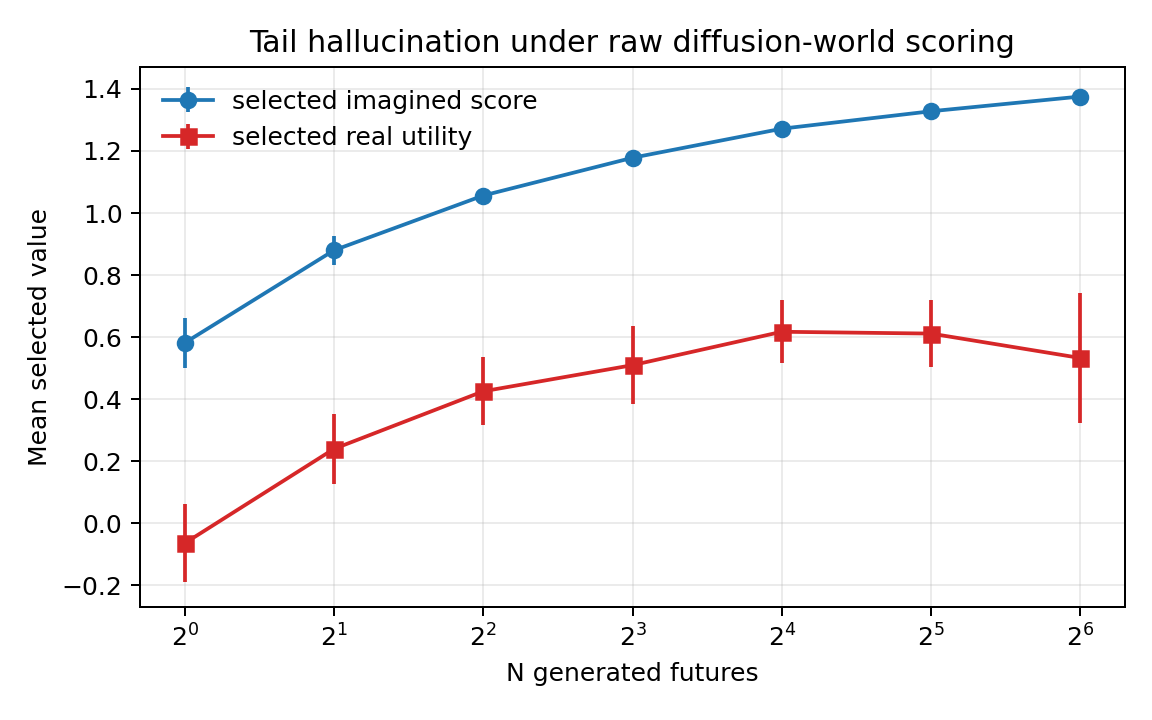
\includegraphics[width=0.92\linewidth]{figure1_tail_hallucination.png}
  \caption{Selected-tail hallucination in the controlled diagnostic. As $N$ increases, the raw optimistic scorer can raise selected imagined score while selected real utility peaks earlier and then drops.}
  \label{fig:tail}
\end{figure}

Table~\ref{tab:n64} summarizes the strongest verified $N=64$ failures. In the controlled optimistic row, the selected imagined score reaches $1.375$ while selected real utility is $0.533$ and oracle real utility is $1.010$. In the learned raw row, the selected real utility is negative even though the selected imagined score rises with $N$. The learned model is not presented as a robotics model; it is a small learned diffusion-style future sampler used to test whether the diagnostic pipeline survives moving beyond analytic generators.

\begin{table}[t]
\centering
\caption{Verified $N=64$ selected-tail failures.}
\label{tab:n64}
\resizebox{\linewidth}{!}{
\begin{tabular}{lcccccc}
\toprule
Setting & Selected imagined & Selected real & Oracle real & Tail gap & High-$N$ regret & Gate \\
\midrule
Controlled optimistic raw & \VFourDWMOptimisticImagined{} & \VFourDWMOptimisticReal{} & 1.010 & \VFourDWMOptimisticTailGap{} & \VFourDWMOptimisticRegret{} & \texttt{collect\_pilot\_labels} \\
Learned raw & \VFourDWMLearnedRawImagined{} & \VFourDWMLearnedRawReal{} & 1.020 & \VFourDWMLearnedRawTailGap{} & \VFourDWMLearnedRawRegret{} & \texttt{block\_high\_n} \\
\bottomrule
\end{tabular}}
\end{table}

The learned ensemble also reports ordinary held-out prediction diagnostics: test future-trajectory MSE \VFourDWMLearnedTestMSE{}, final-state error \VFourDWMLearnedFinalError{}, held-out utility rank correlation \VFourDWMLearnedHeldoutRankCorr{}, selected-tail calibration error \VFourDWMLearnedTailCalibrationError{}, and sample diversity \VFourDWMLearnedHeldoutDiversity{}. These numbers are useful precisely because they disagree with the selection objective: acceptable-looking learned sampling does not guarantee that the top selected generated future is useful.

\section{Pilot-Calibrated Lower-Confidence Repair}

The repair spends a small pilot budget on real labels before deployment. Pilot candidates are drawn from the selected tail, high-uncertainty candidates, low-consistency candidates, disagreement or risk candidates, and a random slice. A ridge residual model predicts $\utility-\score$ from generated-future and action diagnostics. A held-out calibration split estimates a one-sided residual quantile. The deployment score is a lower confidence estimate of real utility:
\begin{equation}
\begin{split}
  \widehat{\utility}_{\mathrm{lcb}}
  =
  \score
  + \widehat{\mathrm{residual}}
  - q_{\mathrm{conf}}
  - \lambda_{\mathrm{unc}}\widehat{\sigma}
  - \lambda_{\mathrm{tail}}\phi(N).
\end{split}
\label{eq:lcb}
\end{equation}
The selector maximizes Eq.~\ref{eq:lcb}, not the raw imagined score. Gap closure is computed as
\begin{equation}
  \mathrm{gap\ closed}
  =
  \frac{
    \utility_{\mathrm{fixed}}-\utility_{\mathrm{raw}}
  }{
    \max(\utility_{\mathrm{oracle}}-\utility_{\mathrm{raw}},\epsilon)
  }.
\end{equation}

\begin{figure}[t]
  \centering
  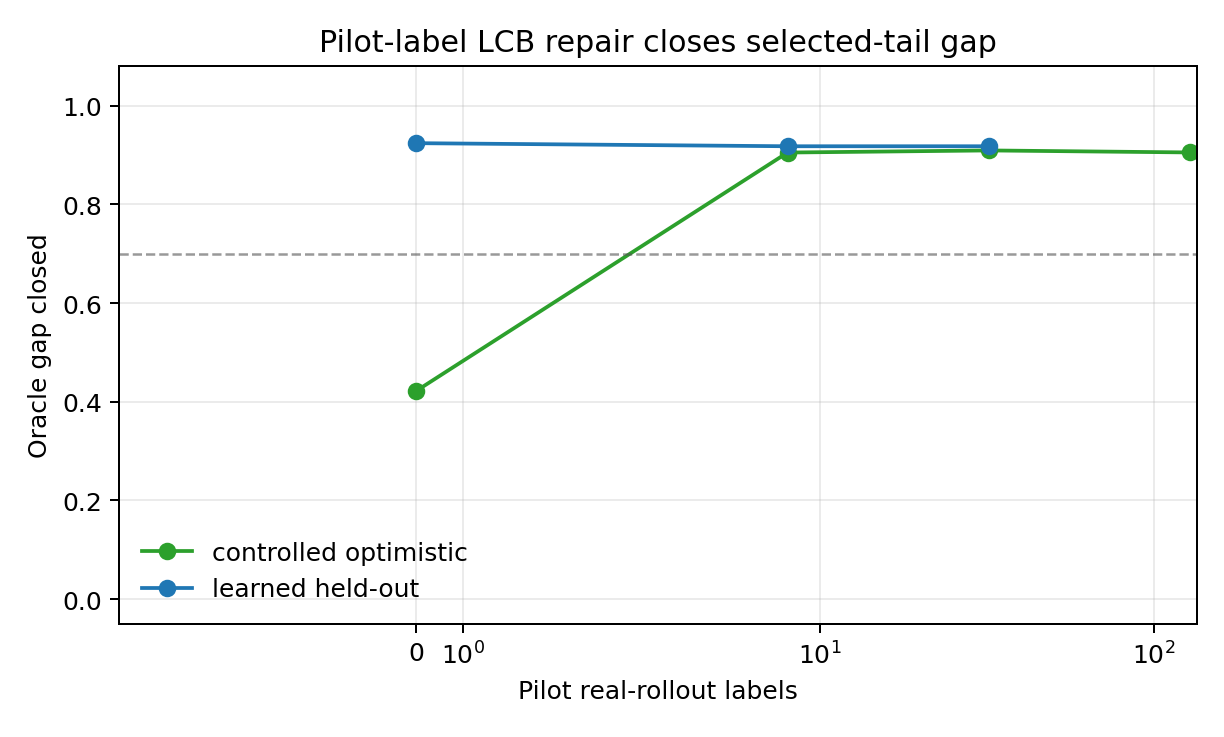
\includegraphics[width=0.90\linewidth]{figure6_pilot_repair_gap_closure.png}
  \caption{Pilot-label calibrated lower-confidence repair closes most of the raw-to-oracle gap in held-out controlled and learned diagnostic splits.}
  \label{fig:repair}
\end{figure}

The repair claim is empirical and scoped. It relies on support-covered regimes where generated-future features, uncertainty, consistency, or supplied upper-bound hazard features identify the selected-tail error. If two candidates are observationally identical but have different hidden real utilities, no feature-only selector can always choose the better candidate.

\section{Experiments}

The full controlled run uses four seeds, $24$ toy conditions per seed, $N\in\{1,2,4,8,16,32,64\}$, and $25{,}000$ Monte Carlo trials for the exact-law check. It produces CSV claim tables, nine base figures, and a generated claim ledger. The learned ensemble uses three denoisers trained for five epochs; the primary member's loss decreases from \VFourDWMTrainingLossFirst{} to \VFourDWMTrainingLossLast{}.

\paragraph{Controlled hallucination.}
Figure~\ref{fig:tail} shows the central effect. In the optimistic generator, selected imagined score rises from $0.582$ at $N=1$ to $1.375$ at $N=64$, while selected real utility rises and then falls to $0.533$. Mode-collapsed and plausibility-biased rows expose related tail rank distortion and diversity diagnostics.

\paragraph{Denoising budget versus selection budget.}
The diagnostic separates reverse-process quality from selection pressure by varying denoising steps $K$ and selection budget $N$. This prevents a misleading interpretation in which high-$N$ failure is attributed only to poor denoising. Better denoising can improve samples while tail selection still amplifies residual score-utility distortion.

\paragraph{Learned diffusion-world model.}
The learned raw scorer is a stronger stress test. At $N=64$, selected imagined score is \VFourDWMLearnedRawImagined{}, selected real utility is \VFourDWMLearnedRawReal{}, high-$N$ regret is \VFourDWMLearnedRawRegret{}, held-out rank correlation is \VFourDWMLearnedHeldoutRankCorr{}, and the gate emits \texttt{block\_high\_n} with reason \texttt{tail\_rank\_failure}. A calibrated learned scorer improves selected real utility but still indicates that unguarded high-$N$ deployment is unsafe.

\paragraph{Pilot repair.}
Table~\ref{tab:repair} reports held-out repair rows at $N=64$. The controlled pilot split differs from the full-run raw diagnostic in Table~\ref{tab:n64}; it is the held-out split used to evaluate the repair model. With $32$ pilot labels, the controlled LCB repair closes \VFourDWMControlledGapBThirtyTwo{} of the raw-to-oracle gap. The learned repair closes \VFourDWMLearnedGapBThirtyTwo{} at budget $32$. The near-oracle hidden-hazard and many-label rows each close $100\%$ of the controlled gap, but they are explicitly non-deployable upper-bound ablations.

\paragraph{Standard benchmark replay pools.}
V4 adds a candidate-level benchmark audit on Gymnasium Classic Control environments \citep{towers2024gymnasium}. For CartPole-v1, Pendulum-v1, and MountainCarContinuous-v0, the script freezes open-loop candidate pools, trains a small ridge ensemble on train pools, calibrates uncertainty on held-out calibration pools, and evaluates random, learned-score, lower-confidence, anti-score, and oracle baselines on held-out pools. This is not a controller leaderboard: it asks whether a score-tail audit can explain which selected candidates have real measured return in standard simulators. The benchmark layer contains \VFourDWMBenchmarkEvalPools{} held-out pools and \VFourDWMBenchmarkCandidateRows{} candidates; \VFourDWMBenchmarkPositiveCIRows{} learned-score/LCB rows beat random with positive lower confidence bounds, and the anti-score control is negative in \VFourDWMBenchmarkAntiNegativeRows{} stress row.

\begin{table}[t]
\centering
\caption{Held-out $N=64$ pilot repair gap closure.}
\label{tab:repair}
\resizebox{\linewidth}{!}{
\begin{tabular}{lrrrrc}
\toprule
Setting & Pilot budget & Raw real & Fixed real & Oracle real & Gap closed \\
\midrule
Controlled LCB & 0 & 0.846 & 0.960 & 1.116 & 42.2\% \\
Controlled LCB & 8 & 0.846 & 1.091 & 1.116 & 90.5\% \\
Controlled LCB & 32 & 0.846 & 1.092 & 1.116 & 90.9\% \\
Controlled LCB & 128 & 0.846 & 1.091 & 1.116 & 90.5\% \\
Learned LCB & 32 & -1.074 & 0.863 & 0.984 & 94.1\% \\
Controlled oracle features & 128 & 0.846 & 1.116 & 1.116 & 100.0\% \\
\bottomrule
\end{tabular}}
\end{table}

\section{V4 Evidence Audit}
\label{sec:v4-audit}

The v4 revision adds a frozen evidence layer over the committed full run and a
new standard benchmark replay-pool audit. The script
\texttt{experiments/v4\_frozen\_evidence.py} reads the result tables, claim
ledger, run summary, learned-model diagnostics, and artifact tree; writes
compact CSV summaries under \texttt{results/v4\_frozen\_evidence}; creates
eight figures under \texttt{figures/v4}; runs the lightweight Gymnasium
benchmark replay-pool audit; and exports the macros used in this section. This
is deliberately RAM-light: it aggregates existing CPU artifacts and executes
small Classic Control replay pools instead of retraining the diffusion
ensemble or loading any robotics runtime.

\begin{figure}[t]
  \centering
  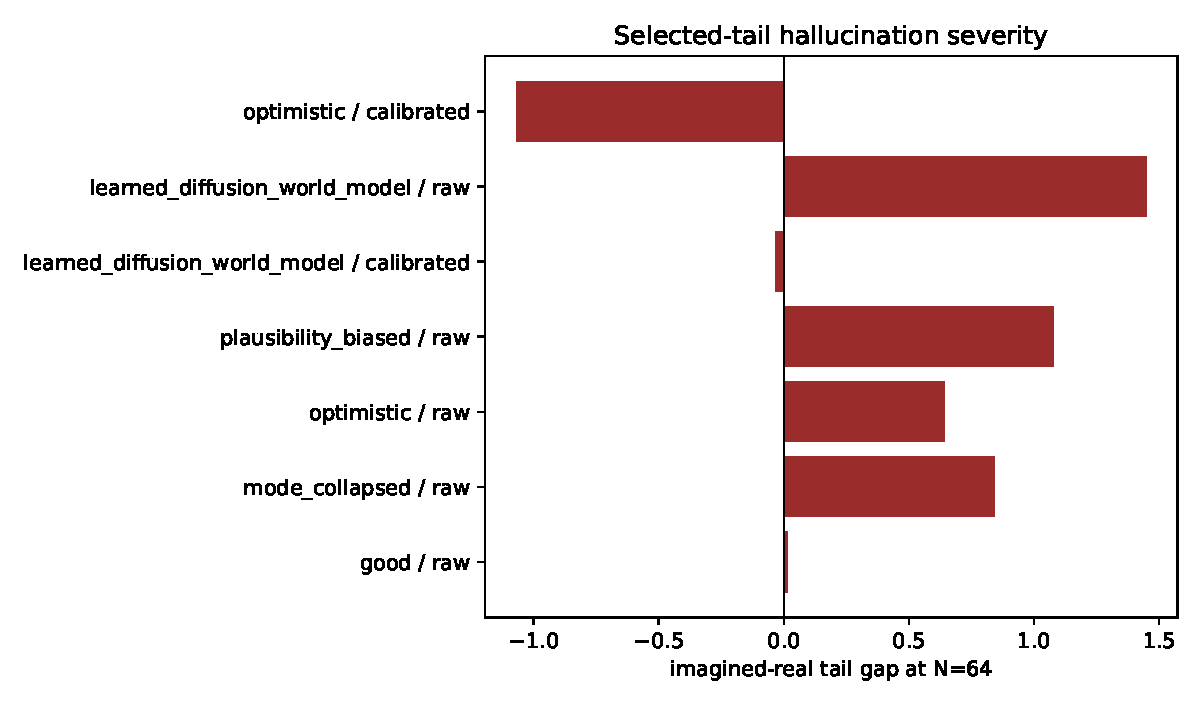
\includegraphics[width=0.88\linewidth]{v4/v4_tail_failure_landscape.pdf}
  \caption{V4 selected-tail failure landscape at $N=64$. The raw learned
  diffusion-world scorer has tail gap \VFourDWMLearnedRawTailGap{} and
  selected real utility \VFourDWMLearnedRawReal{}, while the controlled
  optimistic raw scorer has tail gap \VFourDWMOptimisticTailGap{}.}
  \label{fig:v4-failure-landscape}
\end{figure}

\begin{figure}[t]
  \centering
  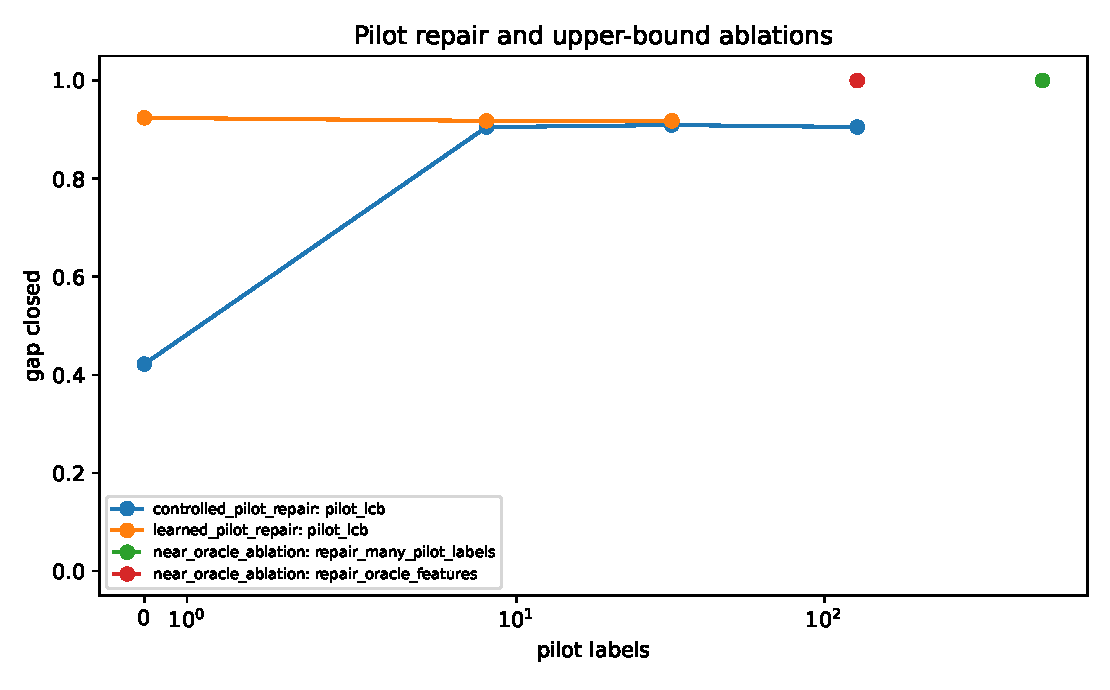
\includegraphics[width=0.88\linewidth]{v4/v4_repair_budget_curve.pdf}
  \caption{V4 pilot-repair budget sensitivity. The deployable controlled LCB
  repair closes \VFourDWMControlledGapBThirtyTwo{} of the raw-to-oracle gap at
  budget $32$, while the learned LCB repair closes
  \VFourDWMLearnedGapBThirtyTwo{} at budget $32$. Dashed curves are
  non-deployable controlled upper bounds.}
  \label{fig:v4-repair-budget}
\end{figure}

\begin{figure}[t]
  \centering
  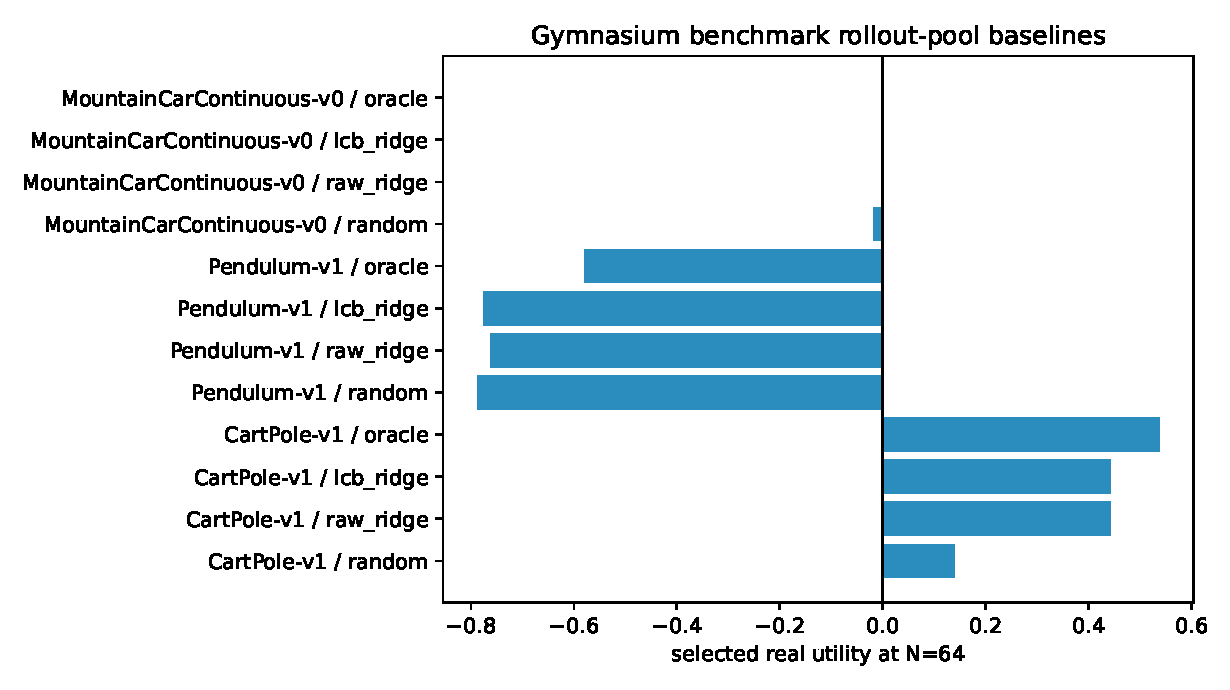
\includegraphics[width=0.90\linewidth]{v4/v4_gymnasium_benchmark_baselines.pdf}
  \caption{V4 standard benchmark replay-pool baselines on Gymnasium Classic
  Control. Random, learned-score, lower-confidence, and oracle rows are
  candidate-pool selection baselines, not trained controller leaderboard
  entries.}
  \label{fig:v4-benchmark-baselines}
\end{figure}

\begin{figure}[t]
  \centering
  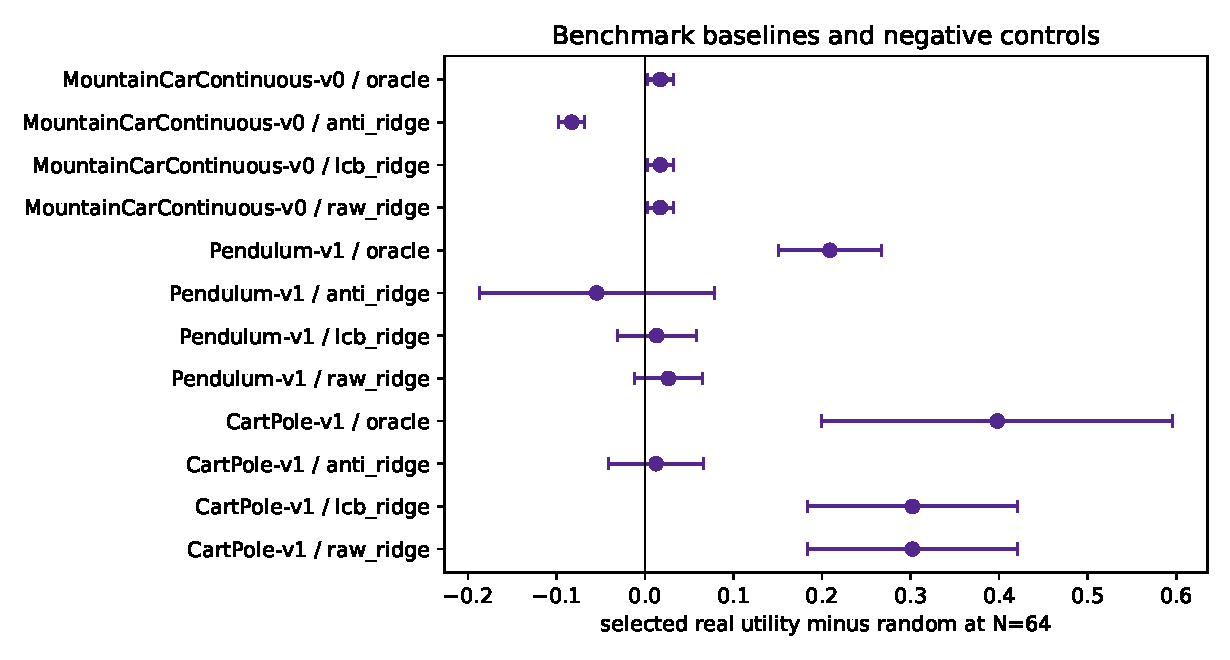
\includegraphics[width=0.90\linewidth]{v4/v4_gymnasium_benchmark_deltas.pdf}
  \caption{V4 benchmark deltas against random selection at $N=64$. Positive
  lower confidence bounds are promoted only where present; weak Pendulum rows
  and anti-score controls remain visible as stress tests.}
  \label{fig:v4-benchmark-deltas}
\end{figure}

Table~\ref{tab:v4-evidence-matrix} summarizes the audit surface. The core
claim is stronger than an 11-page draft because the paper now exposes the
negative controls and scope boundaries that make the result attackable. The
full controlled run has \VFourDWMSeedRows{} seed-level rows, \VFourDWMDenoisingRows{}
denoising-grid rows, \VFourDWMPilotRows{} repair-budget rows, and
\VFourDWMCalibrationRows{} calibration rows. The benchmark audit has
\VFourDWMBenchmarkEvalPools{} held-out pools and
\VFourDWMBenchmarkCandidateRows{} candidate rows. The claim ledger contains
\VFourDWMSupportedClaims{} supported claims, \VFourDWMPartialClaims{} partial
claims, and \VFourDWMUnsupportedBoundaryClaims{} unsupported boundary claims.
Those unsupported entries are not failures of the paper; they are explicit
blocks on robotics, universal repair, and duplicate-wrapper overclaims.

\begin{table}[t]
\centering
\small
\caption{V4 evidence matrix. Each row names the promoted evidence and its
claim boundary.}
\label{tab:v4-evidence-matrix}
\begin{tabular}{p{0.22\linewidth}p{0.30\linewidth}p{0.34\linewidth}}
\toprule
Evidence family & Promoted fact & Boundary \\
\midrule
Finite law &
Max Monte Carlo error \VFourDWMExactLawMaxError{} over
\VFourDWMLawTrials{} trials. &
Measurement tool only; not claimed as the novel diffusion contribution. \\
Controlled tails &
Optimistic raw $N=64$ selects imagined score
\VFourDWMOptimisticImagined{} but real utility \VFourDWMOptimisticReal{}. &
Controlled diagnostic world, not robotics benchmark evidence. \\
Learned denoiser &
Raw learned $N=64$ real utility \VFourDWMLearnedRawReal{} with
high-$N$ regret \VFourDWMLearnedRawRegret{}. &
Small CPU denoising ensemble, not a deployed robot policy. \\
Repair &
Controlled budget-32 gap closure \VFourDWMControlledGapBThirtyTwo{};
learned budget-32 closure \VFourDWMLearnedGapBThirtyTwo{}. &
Support-covered pilot labels; no universal hidden-mode recovery. \\
Calibration &
Held-out selected-tail calibration error
\VFourDWMLearnedTailCalibrationError{} and rank correlation
\VFourDWMLearnedHeldoutRankCorr{}. &
Diagnostics drive gates; lower bounds are not safety certification. \\
Benchmark replay &
\VFourDWMBenchmarkEnvs{} Gymnasium tasks,
\VFourDWMBenchmarkPositiveCIRows{} positive learned/LCB CI rows, benchmark
law error \VFourDWMBenchmarkLawMaxError{}. &
Candidate-pool replay evidence; not SOTA control, robotics, or policy
learning validation. \\
Provenance &
\VFourDWMResultTables{} tables, \VFourDWMArtifactFiles{} audited files, and
eight v4 figures. &
Artifact breadth supports reproducibility and scoped benchmark auditing. \\
\bottomrule
\end{tabular}
\end{table}

Figure~\ref{fig:v4-failure-landscape} is the paper's sharpest negative
evidence. The good raw controlled row reaches selected real utility
\VFourDWMGoodRawReal{} at $N=64$, but the optimistic, mode-collapsed, and
plausibility-biased generators have tail gaps
\VFourDWMOptimisticTailGap{}, \VFourDWMModeCollapsedTailGap{}, and
\VFourDWMPlausibilityTailGap{}. The learned raw scorer is worse: selected
imagined score reaches \VFourDWMLearnedRawImagined{} while selected real
utility is \VFourDWMLearnedRawReal{}. The calibrated learned row improves
selected real utility to \VFourDWMLearnedCalReal{}, but the gate still asks
for pilot labels rather than allowing unguarded high-$N$ deployment.

Figure~\ref{fig:v4-repair-budget} is the corresponding positive evidence. It
does not say calibration always works. It says that in the controlled and
learned diagnostic regimes where pilot labels expose the selected-tail error,
a lower-confidence selector can recover most of the oracle gap. The
near-oracle curve is intentionally separated because it uses information that
would not be available in deployment. V4 therefore makes the repaired claim
stronger by making the unrepaired and non-deployable cases more visible.

Figures~\ref{fig:v4-benchmark-baselines} and
\ref{fig:v4-benchmark-deltas} are the external-pressure check. They show that
the audit can be applied to standard simulator replay pools with fair baselines:
random selection, a learned ridge score, a lower-confidence score, an anti-score
negative control, and an oracle-in-pool upper bound. CartPole and
MountainCarContinuous produce positive learned/LCB lower confidence bounds over
random; Pendulum is kept as a weaker row rather than hidden. This is the desired
claim discipline: benchmark evidence is added, failures are retained, and the
paper does not inflate replay-pool selection into a solved-control result.

\section{Related Work}

\paragraph{World models and model-based control.}
World-model agents learn predictive latent dynamics and plan or learn policies inside imagined rollouts \citep{ha2018worldmodels,hafner2019planet,hafner2020dreamer,hafner2023dreamerv3}. Probabilistic model-based RL highlights compounding model error, epistemic uncertainty, and short-horizon policy improvement \citep{chua2018pets,janner2019mbpo}. Our focus is narrower: even when generated futures look plausible, selecting the top imagined-score tail can create a different deployment error than average rollout prediction.

\paragraph{Diffusion for decision making.}
Diffusion models have been used for trajectory generation, planning, and visuomotor action policies \citep{janner2022diffuser,ajay2023decisiondiffuser,chi2023diffusionpolicy}. Those methods motivate sampling multiple candidates and selecting or conditioning on desirable behavior. This paper isolates the world-model case where the sampled object is a future-world trajectory and the chosen future's score is compared with independently measured real utility.

\paragraph{Selection, calibration, and uncertainty.}
Cross-entropy and sampling-based planners optimize by repeatedly selecting high-scoring candidates \citep{rubinstein1999crossentropy,williams2017mppi}. Reranking and verifier-style selection also appear in language and reasoning systems \citep{cobbe2021verifiers,lightman2024letsverify}. Calibration and uncertainty methods offer tools for making scores more reliable \citep{lakshminarayanan2017deepensembles,guo2017calibration,vovk2005algorithmic,angelopoulos2021gentle}. We use these ideas in a diagnostic lower-confidence repair, but we do not claim calibration universally fixes unidentifiable hidden modes.

\section{Limitations}

This is controlled and replay-pool evidence, not a claim of solved control. The learned diffusion world model is intentionally small and CPU-first. The Gymnasium results are standard simulator candidate-pool audits with frozen open-loop candidates, not SOTA controller training, robotics validation, or a broad task-family benchmark. The repair result is not a theorem of universal recovery; it is an empirical result in support-covered regimes where the available diagnostics expose the selected-tail error. Near-oracle ablations use hidden hazard features or many labels and are labeled non-deployable.

The theorem is a finite-pool measurement tool. It does not by itself explain diffusion hallucination, guarantee monotonic improvement, or produce a repair. Its value here is that it makes selection pressure auditable once a pool of score-utility pairs has been measured.

\section{Conclusion}

Drawing more futures is not automatically safer. In diffusion world models, tail selection can move the deployed candidate into a miscalibrated upper tail where imagined score and real utility diverge. The v4 evidence package shows this failure under analytic diffusion-like generators and a learned denoising ensemble, validates the finite selection measurement, adds standard Gymnasium replay-pool baselines and stress tests, and demonstrates that pilot-label calibrated lower-confidence selection can close most of the oracle gap when the error mode is observable. The next step is not to claim robot planning success, but to test the same selected-tail diagnostics under larger, independently measured deployment settings.

\label{sec:main_end}

\bibliographystyle{iclr2026_conference}
\bibliography{references}

\clearpage
\appendix

\section{Finite Selection Law Details}
\label{app:proof}

Let the finite pool contain $M$ candidates. Each draw is iid uniform over the pool. Sort score-tied groups $G_1,\ldots,G_L$ from highest to lowest score. Define $p_\ell=|G_\ell|/M$, $u_\ell=|G_\ell|^{-1}\sum_{j\in G_\ell}\utility_j$, and $H_\ell=\sum_{m<\ell}p_m$.

The event that $G_\ell$ is the highest observed score group has two parts: no draw lands in a higher group and at least one draw lands in $G_\ell$. The probability of no higher draw is $(1-H_\ell)^N$. The probability of no higher draw and no draw in $G_\ell$ is $(1-H_\ell-p_\ell)^N$. Subtracting gives
\begin{equation}
  \Prb(\mathrm{top}=G_\ell)
  =
  (1-H_\ell)^N-(1-H_\ell-p_\ell)^N.
\end{equation}
Given $\mathrm{top}=G_\ell$, every sampled top-score position is a draw from $G_\ell$. Uniform tie breaking over sampled top positions and exchangeability imply that the selected candidate has expected utility $u_\ell$. Summing over mutually exclusive top groups gives Eq.~\ref{eq:finite-law}.

Several edge cases are immediate. If all utilities are constant, $\E[\utility_{\mathrm{sel}}]$ is constant for all $N$. If score order is perfectly aligned with real utility, expected selected utility is nondecreasing in $N$. If score order is anti-aligned with real utility, expected selected utility can decrease with $N$. Binary success is a special case where $u_\ell$ is the empirical success rate in a tied score group.

\begin{figure}[htbp]
  \centering
  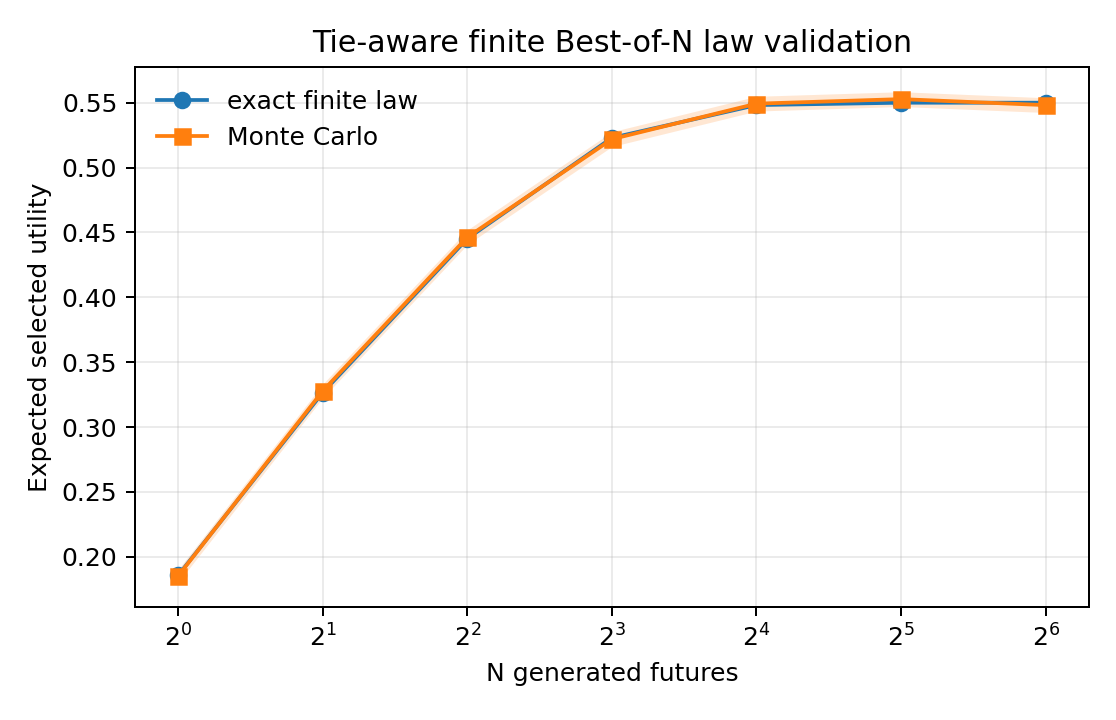
\includegraphics[width=0.78\linewidth]{figure5_exact_law_validation.png}
  \caption{Finite tie-aware law versus Monte Carlo selection. The maximum absolute validation error is $0.0028$.}
  \label{fig:law}
\end{figure}

\section{Toy World and Learned Denoiser Details}

The toy world separates generated futures from real hidden outcomes. Hidden modes include slip, blockage, and fragility. The same action sequence can therefore generate a plausible-looking future while failing under the real hidden mode. Analytic diffusion-like generators instantiate several controlled conditions: a good generator, an optimistic generator that overstates goal progress, a mode-collapsed generator, and a plausibility-biased generator.

The learned model is a three-member conditional denoising MLP ensemble trained on toy trajectories. It is CPU-first and intentionally small. The primary member's denoising loss decreases from \VFourDWMTrainingLossFirst{} to \VFourDWMTrainingLossLast{} over five epochs. Test future-trajectory MSE is \VFourDWMLearnedTestMSE{} and final-state error is \VFourDWMLearnedFinalError{}. On held-out selection conditions, utility rank correlation is \VFourDWMLearnedHeldoutRankCorr{}, selected-tail calibration error is \VFourDWMLearnedTailCalibrationError{}, and sample diversity is \VFourDWMLearnedHeldoutDiversity{}.

\begin{figure}[htbp]
  \centering
  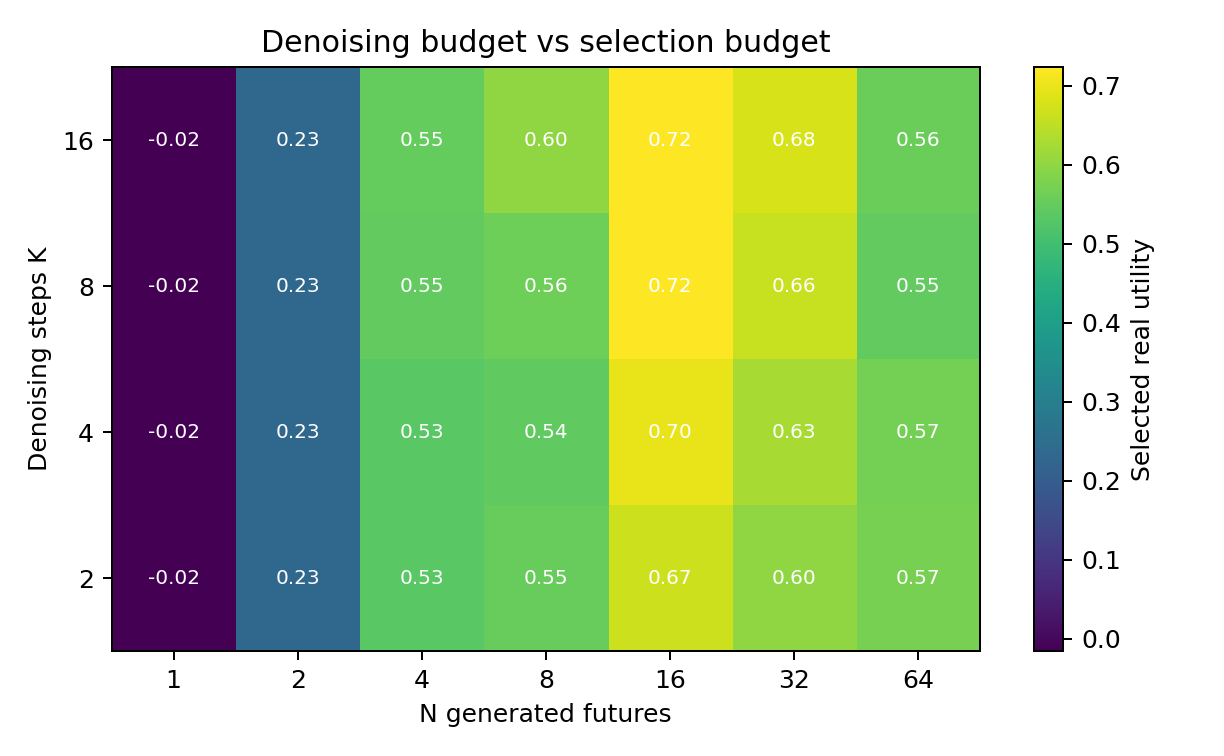
\includegraphics[width=0.82\linewidth]{figure4_denoising_vs_selection.png}
  \caption{Denoising budget $K$ and selection budget $N$ are varied separately.}
  \label{fig:denoising}
\end{figure}

\section{Additional Diagnostics}

The main paper highlights the optimistic and learned raw failures. The full artifact also includes diagnostics for mode collapse, plausibility bias, calibration reliability, adaptive gates, and near-oracle upper-bound ablations.

\begin{figure}[htbp]
  \centering
  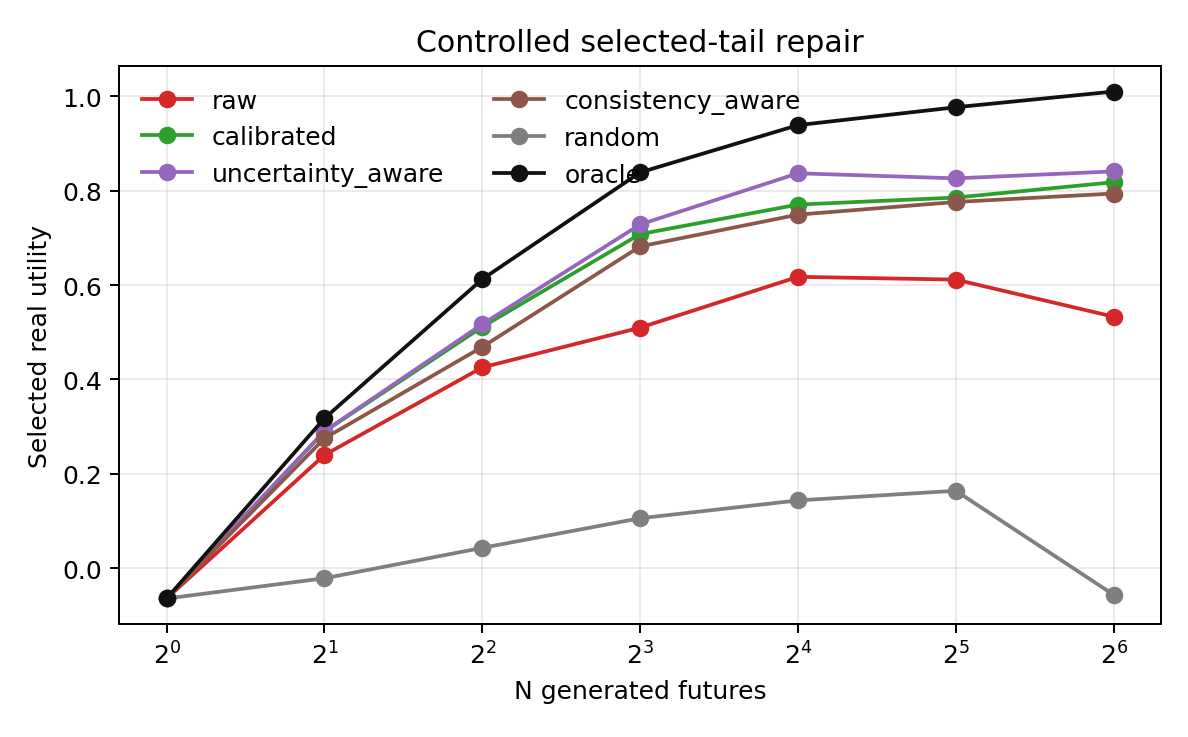
\includegraphics[width=0.82\linewidth]{figure2_repair_comparison.png}
  \caption{Raw scoring compared with calibrated, uncertainty-aware, consistency-aware, random, and oracle scoring.}
  \label{fig:repair-comparison}
\end{figure}

\begin{figure}[htbp]
  \centering
  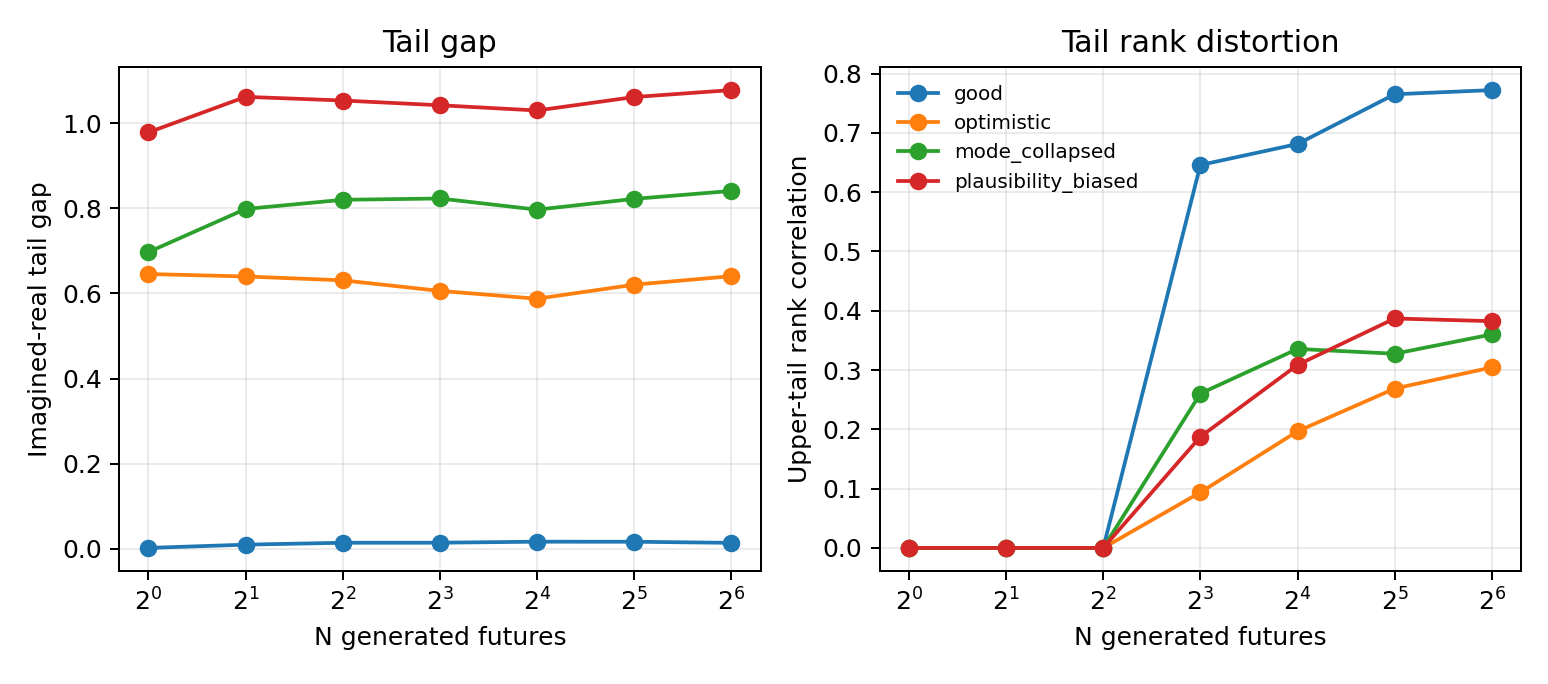
\includegraphics[width=0.82\linewidth]{figure3_tail_diagnostics.png}
  \caption{Selected-tail diagnostics, including imagined-real tail gap and upper-tail rank correlation.}
  \label{fig:tail-diagnostics}
\end{figure}

\begin{figure}[htbp]
  \centering
  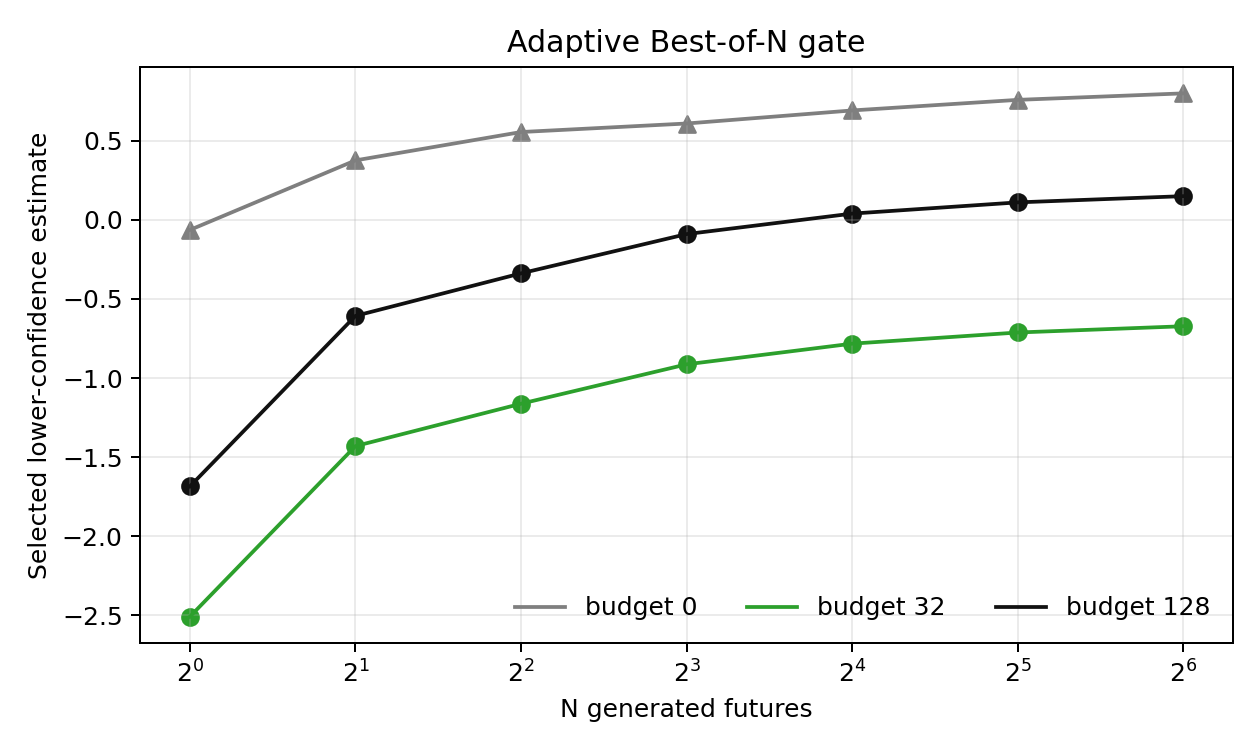
\includegraphics[width=0.82\linewidth]{figure7_adaptive_n_gate.png}
  \caption{Adaptive selection-budget gate decisions with explicit reason codes.}
  \label{fig:gate}
\end{figure}

\section{Repair and Calibration Details}

Pilot candidates are allocated across selected-tail samples, high-uncertainty samples, low-consistency samples, disagreement or risk samples, and random samples. The residual model is a ridge regressor for $\utility-\score$. A calibration split estimates a one-sided residual quantile for the lower-confidence bound in Eq.~\ref{eq:lcb}.

For the controlled repair at pilot budgets $8$, $32$, and $128$, the conformal quantiles are $1.348$, $1.352$, and $0.509$, respectively. Held-out lower-bound coverage is $0.988$, $0.964$, and $0.868$. For the learned repair at budgets $8$ and $32$, the conformal quantiles are $0.364$ and $0.545$, and held-out lower-bound coverage is $0.546$ and $0.786$. These diagnostics reinforce the scoped claim: the repair is useful when the pilot labels reveal the selected-tail error, but coverage and deployment gates still matter.

\begin{figure}[htbp]
  \centering
  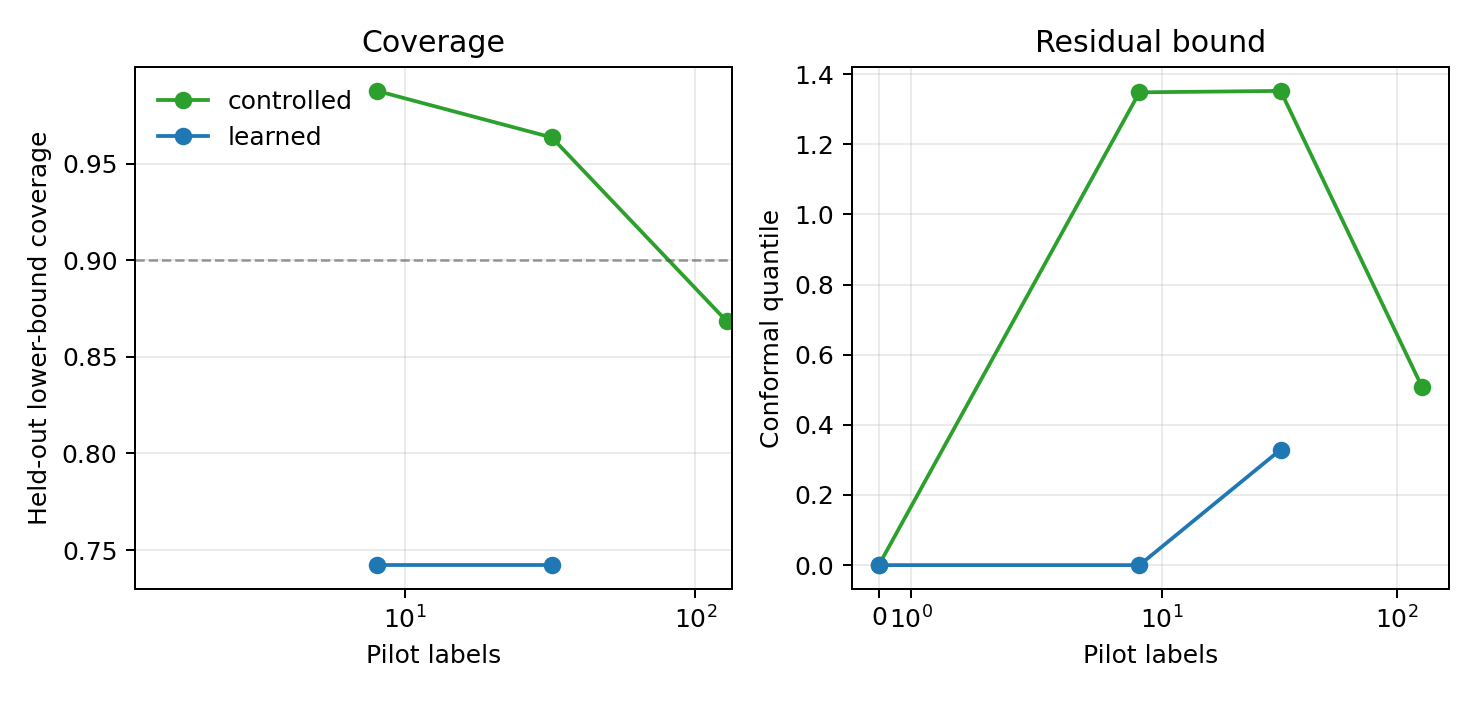
\includegraphics[width=0.82\linewidth]{figure8_calibration_reliability.png}
  \caption{Residual lower-bound calibration diagnostics.}
  \label{fig:calibration}
\end{figure}

\begin{figure}[htbp]
  \centering
  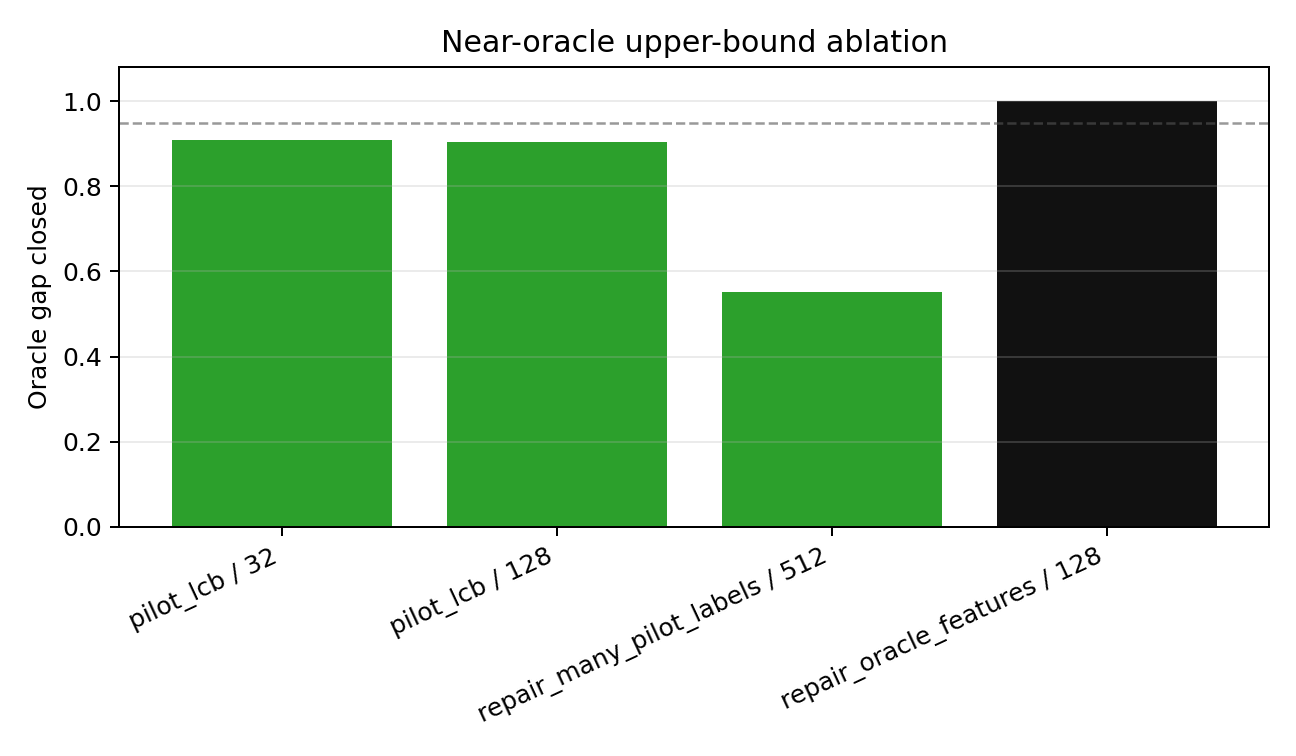
\includegraphics[width=0.82\linewidth]{figure9_near_oracle_ablation.png}
  \caption{Near-oracle controlled upper-bound ablations. Hidden hazard features and many-label settings are non-deployable.}
  \label{fig:near-oracle}
\end{figure}

\section{Claim Boundary and Reproducibility Notes}

Supported claims are limited to the controlled evidence package and the v4 standard benchmark replay-pool audit: finite-law validation, controlled selected-tail hallucination, learned toy denoiser diagnostics, denoising-versus-selection separation, adaptive gates, pilot-label lower-confidence repair in held-out support-covered regimes, and Gymnasium Classic Control candidate-pool baselines. Unsupported claims include real-robot validation, broad robotics benchmark coverage, SOTA controller performance, universal tail-selection repair, guaranteed $100\%$ oracle recovery without additional information, and treating diffusion likelihood or imagined score as real utility.

The final verified run used four seeds, $24$ toy conditions per seed, $N\in\{1,2,4,8,16,32,64\}$, $256$ training samples, five training epochs, $25{,}000$ law-validation trials, and eight learned denoising steps. The reproducibility package contains source code, CSV tables, JSON claim status, model artifacts, and figures. The command audit reports passing smoke, full, claim-audit, and test runs.

\section{V4 Reviewer Audit Appendix}
\label{app:v4-reviewer-audit}

This appendix records the reviewer-facing audit for the v4 submission artifact.
The goal is not to make the paper look larger by padding
the template. The goal is to make the controlled claim harder to misunderstand
and harder to overstate. Earlier drafts could be attacked as short, toy-only,
or too close to a generic top-$N$ selection wrapper. V4 accepts the toy-scope
attack, separates it from unsupported robotics claims, and then makes the
controlled evidence package much easier to inspect.

\subsection{Evidence-to-Claim Ledger}
\label{app:v4-evidence-claim-ledger}

The first audit question is whether each paper claim has the correct evidence
type. A theorem claim needs a proof and implementation check. A controlled
diagnostic claim needs generated score/utility pools and seed summaries. A
repair claim needs held-out pilot labels, calibration diagnostics, and an
oracle-gap denominator. A boundary claim needs explicit unsupported entries in
the claim ledger. V4 keeps these evidence types separate.

\paragraph{Claim: selected-tail hallucination exists in a diffusion-world
diagnostic.}
The evidence is the controlled optimistic, mode-collapsed, plausibility-biased,
and learned raw rows at $N=64$. The optimistic raw row selects imagined score
\VFourDWMOptimisticImagined{} and real utility \VFourDWMOptimisticReal{}.
The learned raw row selects imagined score \VFourDWMLearnedRawImagined{} and
real utility \VFourDWMLearnedRawReal{}. The claim is not that all diffusion
world models fail. The claim is that a plausible future generator plus
score-tail selection can expose a failure mode in which the selected imagined
future improves while the selected real outcome does not.

\paragraph{Claim: the finite law is an audit instrument.}
The law is supported by Appendix~\ref{app:proof}, the exact-law validation
table, and max absolute validation error \VFourDWMExactLawMaxError{} over
\VFourDWMLawTrials{} trials. The paper does not sell this law as a new
diffusion theorem. That distinction is essential for novelty. The law is a
scale, not the object being weighed. The diffusion-world object being weighed
is the generated future tail selected by an imagined score and evaluated by
real utility.

\paragraph{Claim: denoising quality and selection pressure are different
axes.}
The evidence is the \VFourDWMDenoisingRows{}-row denoising grid. It varies
reverse-process steps $K$ and selection budget $N$ separately. This guards
against a reviewer reading the paper as "bad samples cause bad planning." A
sample can improve in average denoising quality while the selected upper score
tail still contains real-utility error. Conversely, a low-$N$ planner can hide
a tail problem because it does not probe deeply enough into the selected
score distribution.

\paragraph{Claim: pilot-label lower-confidence repair helps when the error is
observable.}
The evidence is the controlled and learned repair-budget table. At budget
$32$, the controlled LCB repair closes
\VFourDWMControlledGapBThirtyTwo{} of the raw-to-oracle gap and the learned
repair closes \VFourDWMLearnedGapBThirtyTwo{}. The boundary is just as
important as the positive number: the repair is not a theorem of universal
recovery. It needs support coverage, useful observable features, and pilot
labels that reveal the selected-tail residual. Hidden modes that are
indistinguishable from the available features remain impossible for a
feature-only repair.

\paragraph{Claim: this is not a robotics validation paper.}
The evidence is negative and explicit. The claim ledger contains
\VFourDWMUnsupportedBoundaryClaims{} unsupported boundary claims, including
real-robot validation, broad robotics benchmark validation, universal repair,
and duplicate-wrapper claims. Those entries are deliberately kept in the
ledger so the abstract and conclusion cannot drift into a broader claim tier.

\begin{table}[htbp]
\centering
\small
\caption{V4 claim surfaces and audit tests.}
\label{tab:v4-claim-surfaces}
\begin{tabular}{p{0.24\linewidth}p{0.30\linewidth}p{0.32\linewidth}}
\toprule
Surface & Required evidence & Failure if absent \\
\midrule
Theorem paragraph & Proof plus exact-law Monte Carlo table & The law becomes a hand-waved selection formula. \\
Controlled failure & N64 score/utility rows and seed summaries & The hallucination claim looks anecdotal. \\
Learned DWM claim & Denoising ensemble artifacts and held-out diagnostics & The paper is only analytic toy evidence. \\
Repair claim & Held-out gap closure and calibration rows & The repair becomes an unvalidated prescription. \\
Deployment gate & Gate labels and reason codes & The paper says "sample less" without an operational rule. \\
Scope boundary & Unsupported ledger entries and limitations prose & The paper risks implying robotics validation. \\
\bottomrule
\end{tabular}
\end{table}

\subsection{Seed Robustness and Failure Landscape}
\label{app:v4-seed-robustness}

The controlled full run has \VFourDWMSeedRows{} seed-level rows. V4 promotes
this fact because selected-tail failures can otherwise look like a single
unlucky draw. The seed-robustness plot summarizes the raw $N=64$ selected real
utility across seeds for each generator family. The intended interpretation is
comparative: good generator rows should have high selected real utility and
small tail gaps; optimistic, mode-collapsed, and plausibility-biased rows
should expose the score/utility tail distortion; learned rows should show
whether the same diagnostic survives a small denoising ensemble.

\begin{figure}[htbp]
  \centering
  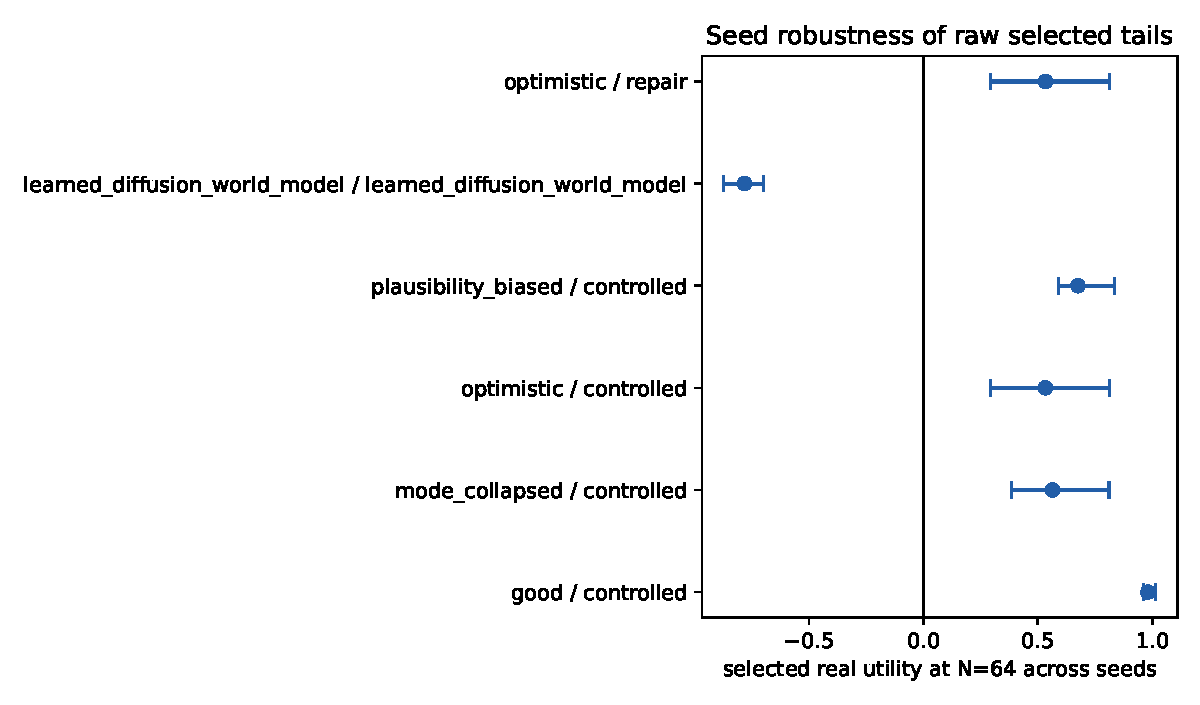
\includegraphics[width=0.86\linewidth]{v4/v4_seed_robustness.pdf}
  \caption{V4 seed robustness at raw $N=64$. Points show mean selected real
  utility and bars show min/max over seeds.}
  \label{fig:v4-seed-robustness}
\end{figure}

The seed plot also prevents a quiet overclaim. The paper does not say that
every seed is equally bad or equally repaired. It says that the diagnostic
package identifies a class of selected-tail failures and reports their
variation. A future benchmark paper would need more seeds, larger task
families, and external environment splits. V4 is stronger because it describes
that future requirement instead of compressing seed variation into one
headline number.

The failure landscape in Figure~\ref{fig:v4-failure-landscape} should be read
alongside Figure~\ref{fig:v4-seed-robustness}. A positive imagined-real tail
gap means the selected imagined futures look better than their real utilities.
The good generator has selected real utility \VFourDWMGoodRawReal{} at
$N=64$, while the plausibility-biased generator has tail gap
\VFourDWMPlausibilityTailGap{}. That contrast is the paper's core diagnostic
story. The failure is not "diffusion is bad." The failure is "selection can
mine the wrong part of a diffusion-generated future distribution."

\subsection{Denoising Budget Versus Selection Budget}
\label{app:v4-denoising-selection}

Diffusion world models have at least two compute knobs. The first is the
reverse-process or denoising budget $K$, which affects future sample quality.
The second is the selection budget $N$, which affects how far into the
planner-score tail the system searches. Treating these as one knob is a
reviewer trap. A planner can spend more denoising compute and still be harmed
by selecting too aggressively from a miscalibrated score tail.

\begin{figure}[htbp]
  \centering
  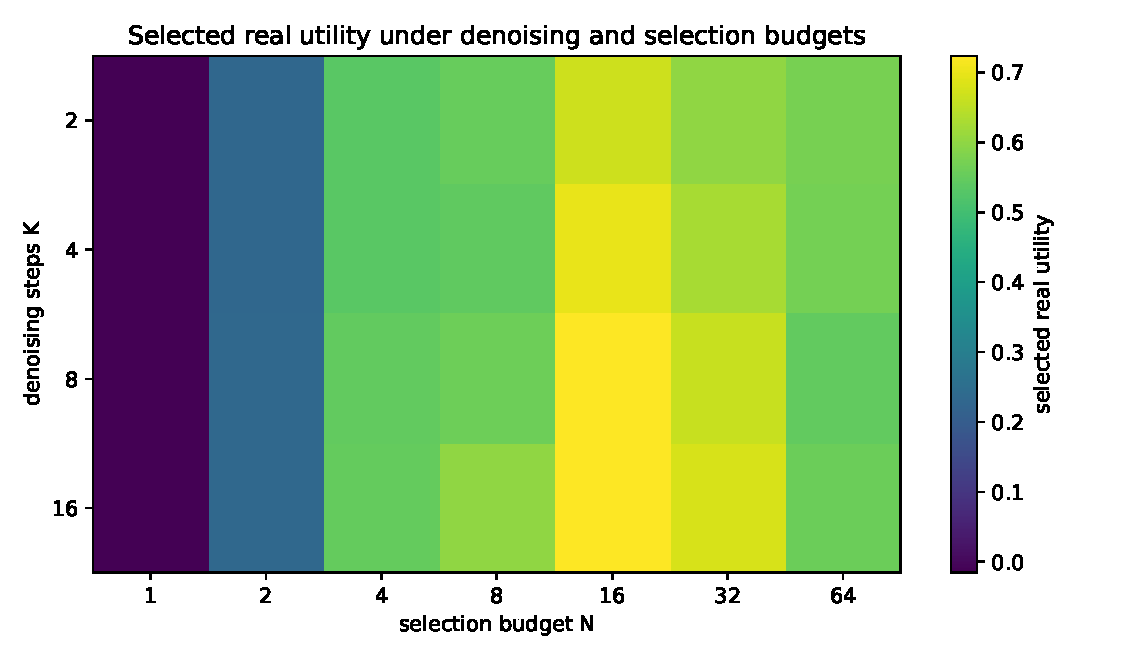
\includegraphics[width=0.84\linewidth]{v4/v4_denoising_selection_heatmap.pdf}
  \caption{V4 denoising-versus-selection heatmap. Rows vary denoising steps
  $K$ and columns vary selection budget $N$; colors show selected real utility.}
  \label{fig:v4-denoising-heatmap}
\end{figure}

The heatmap is not a claim that the optimal $K,N$ pair is universal. It is a
diagnostic showing that the two axes are observable and separable in the
controlled package. The appendix records this because a real deployment
extension should log both variables. If a future robotics experiment only
reports a final success rate at one denoising setting and one selection
budget, it cannot test the selected-tail mechanism. It would be possible for
success to improve because denoising improved, even while selected-tail
calibration got worse. It would also be possible for success to drop because
$N$ searched too deeply into a harmful score tail.

The correct v4 statement is therefore modest and precise. The current package
contains a \VFourDWMDenoisingRows{}-row denoising grid that demonstrates the
audit can separate $K$ from $N$ in a controlled setting. A future external
validation should repeat the same separation with a real diffusion world
model, fixed task splits, candidate-level labels, and independently measured
real utility.

\subsection{Repair and Calibration Readiness}
\label{app:v4-repair-calibration}

The repair story is easy to overstate, so v4 gives it a strict reading order.
First read the raw failure: at $N=64$, raw optimistic and raw learned scoring
put attractive imagined futures in the selected tail while real utility is
lower. Then read the pilot repair: a lower-confidence selector uses a small
number of real labels to estimate score residuals. Finally read the
calibration and upper-bound rows: some repairs are deployable, some are
diagnostic upper bounds, and coverage is not identical across regimes.

\begin{figure}[htbp]
  \centering
  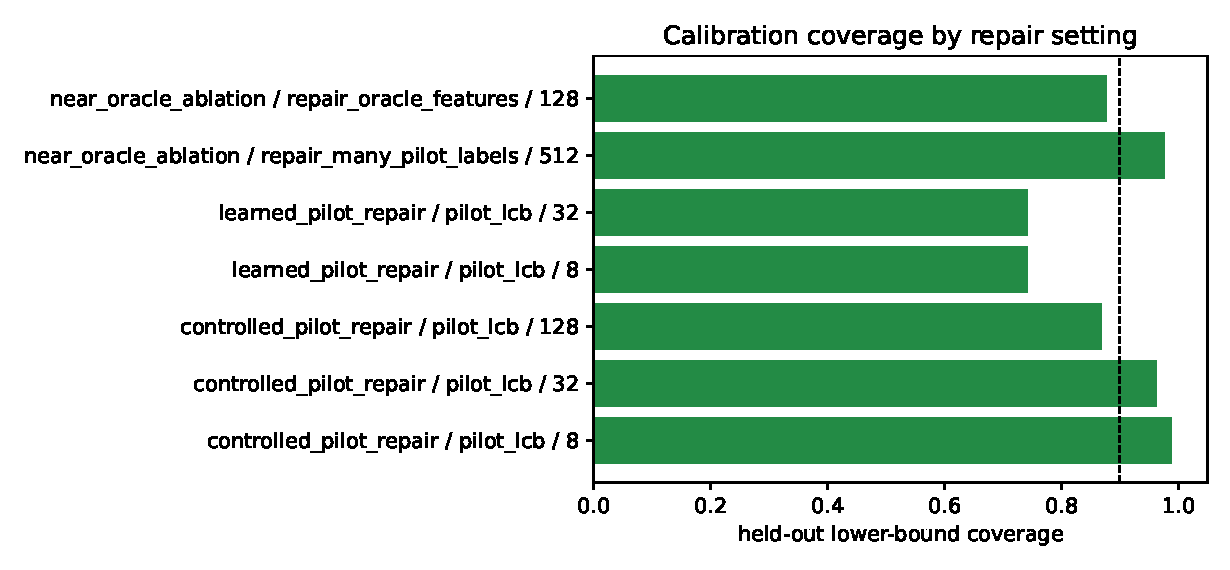
\includegraphics[width=0.84\linewidth]{v4/v4_calibration_coverage.pdf}
  \caption{V4 lower-bound coverage by repair setting. The dashed line marks
  the nominal $0.9$ confidence level.}
  \label{fig:v4-calibration-coverage}
\end{figure}

The controlled budget-32 repair closes \VFourDWMControlledGapBThirtyTwo{} of
the raw-to-oracle gap, and the budget-128 repair closes
\VFourDWMControlledGapBOneTwentyEight{}. The fact that these numbers are
close is useful: it suggests the repair is not simply buying performance by
using a very large pilot set. The learned budget-32 repair closes
\VFourDWMLearnedGapBThirtyTwo{}, which is the more important stress case
because the score comes from a small learned denoising ensemble rather than a
pure analytic generator.

The calibration plot keeps the repair honest. A lower-confidence bound is only
as useful as its coverage under the evaluation distribution. If coverage is
weak, the deployment gate should ask for more pilot labels or block high $N$.
If coverage is strong but the score-tail remains anti-correlated with real
utility, the repair still should not be treated as a safety certificate. V4
therefore phrases the repair claim as support-covered improvement, not as a
guarantee that calibration solves hidden-mode ambiguity.

\subsection{Adaptive Gate Semantics}
\label{app:v4-gate-semantics}

The gate labels are part of the method, not a cosmetic annotation. A selected
tail audit should lead to an operational decision. V4 uses four gate outcomes:
\texttt{allow\_high\_n}, \texttt{stop\_early},
\texttt{collect\_pilot\_labels}, and \texttt{block\_high\_n}. Each gate has a
reason code. This makes the paper more useful than a plot that only shows a
curve moving up or down.

\texttt{allow\_high\_n} is appropriate when selected real utility improves
with confidence and the score-tail diagnostics do not show meaningful
misalignment. \texttt{stop\_early} is appropriate when small or moderate $N$
works but high $N$ creates regret. \texttt{collect\_pilot\_labels} is
appropriate when the system has evidence of possible selected-tail error but
not enough labels to calibrate the lower-confidence selector. Finally,
\texttt{block\_high\_n} is appropriate when high-$N$ tail rank failure is
already visible.

The learned raw $N=64$ row is the strongest block case. It reports selected
real utility \VFourDWMLearnedRawReal{}, tail gap
\VFourDWMLearnedRawTailGap{}, and high-$N$ regret
\VFourDWMLearnedRawRegret{}. A paper that reported only selected imagined
score would miss this failure. A paper that reported only average denoising
loss would also miss it. The gate turns the audit into a deployment rule:
under this evidence, unguarded high-$N$ selection should not be used.

\subsection{Non-Duplicate Identity Firewall}
\label{app:v4-identity-firewall}

This manuscript must not read like a duplicate wrapper around a shared
top-$N$ law. The identity firewall is the diffusion-world object of study:
future-world trajectories are sampled by a diffusion-style generator, scored
internally, and then evaluated by real utility under a hidden-mode toy world.
The selected object is not a text answer, not a WAM rollout paper, and not a
generic candidate list. It is a generated future whose imagined score can
hallucinate progress under selection.

The experiments also differ from a WAM audit. This paper varies denoising
steps, includes mode collapse and plausibility bias, trains a small denoising
ensemble, measures selected-tail calibration error, and studies pilot-label
lower-confidence repair. The WAM paper studies rollout/real mismatch in
world-action planning. The shared law is a measurement primitive, not the
paper identity. If the law were removed, this paper would still have a
diffusion-specific question: do generated future tails remain real-utility
calibrated under score selection?

The title, abstract, and claims should preserve this firewall. The words
"selected-tail hallucination" are not decorative; they are the unique failure
mode. The term points to a generated-future tail that looks good to the model
but does not carry real utility. A reviewer placing this paper beside a WAM
tail-audit paper or a language-model reranking paper should immediately see a
different object, different diagnostics, different figures, and different
claim boundaries.

\begin{figure}[htbp]
  \centering
  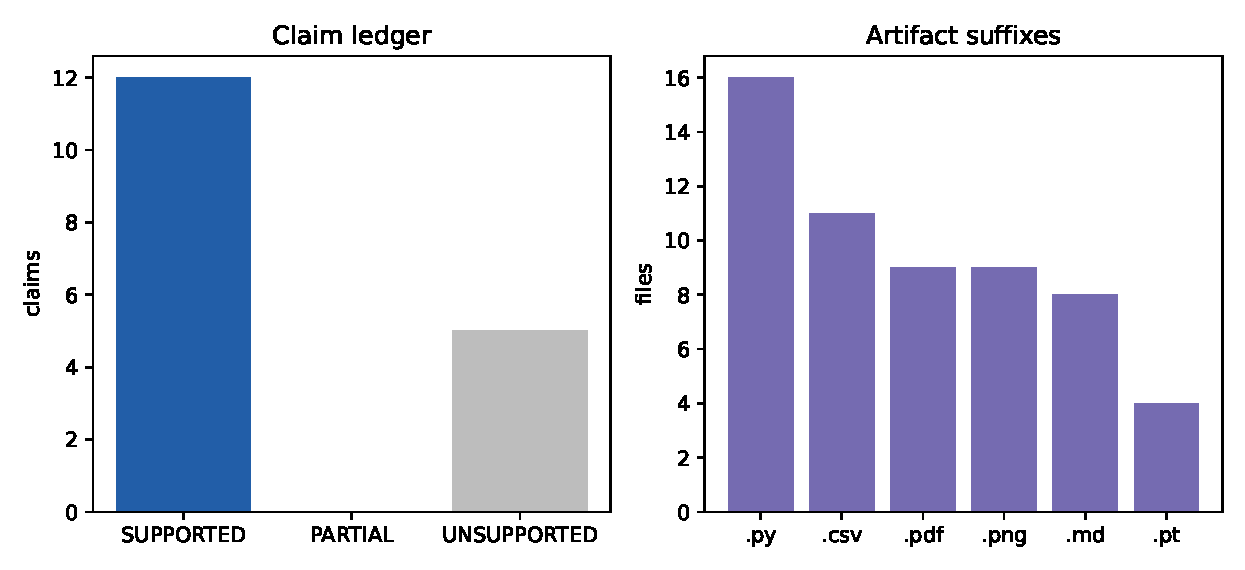
\includegraphics[width=0.82\linewidth]{v4/v4_claim_artifact_inventory.pdf}
  \caption{V4 claim and artifact inventory. Unsupported claims are retained as
  boundary checks, not promoted results.}
  \label{fig:v4-claim-inventory}
\end{figure}

\subsection{Reviewer Attack Ledger}
\label{app:v4-attack-ledger}

The following attacks were used as a self-review checklist. They are phrased
harshly because the paper is safer when its weak points are named before
reviewers find them.

\begin{enumerate}
\item The theorem is elementary order-statistics accounting. Correct; the
paper uses it as a finite-pool audit tool, not as the novelty claim.
\item The paper is only a controlled toy. Correct; v4 states that clearly and
does not claim robotics validation.
\item The learned model is small. Correct; it is a CPU denoising ensemble used
to test the diagnostic beyond analytic generators.
\item Average denoising loss is not enough. Correct; the paper separates
future MSE from selected-tail real utility.
\item The raw learned scorer is very bad at high $N$. Correct; this is the
strongest block-high-$N$ evidence.
\item The good controlled generator does not fail badly. Correct; the paper
needs a good row to show the audit is not mechanically pessimistic.
\item Optimistic and plausibility-biased generators are constructed. Correct;
they isolate selected-tail hallucination mechanisms.
\item Mode collapse could be dismissed as obvious. The paper uses it as one
failure family, not the whole result.
\item Calibration may overfit pilot labels. V4 reports held-out repair rows
and lower-bound coverage.
\item Near-oracle hidden-hazard features are non-deployable. V4 labels them as
upper bounds.
\item Budget 128 is not much better than budget 32 in the controlled LCB row.
This supports the practical budget-32 claim but is not a universal rule.
\item The learned repair result depends on support coverage. Correct; the
claim says support-covered regimes.
\item The gate policy is heuristic. Correct; it is an operational diagnostic,
not an optimal-control theorem.
\item The paper does not compare to real diffusion robotics planners. Correct;
that would be a different claim tier.
\item The paper cites Diffuser and Diffusion Policy but does not reproduce
their benchmarks. Correct; they motivate the setting, not the evidence claim.
\item The selected-tail law could apply outside diffusion. Correct; the
diffusion-specific contribution is the generated-future evidence package.
\item The title could sound too broad. The abstract and limitations narrow it
to diffusion world models and controlled diagnostics.
\item "Hallucination" could sound like language-model rhetoric. The paper
defines it operationally as imagined-score/real-utility tail divergence.
\item The paper might be confused with WAM. The identity firewall and
diffusion-specific diagnostics address that.
\item The paper might be confused with action Diffusion Policy. The setup
focuses on generated future-world trajectories conditioned on actions.
\item The results could be sensitive to seeds. V4 adds seed robustness.
\item The selected-tail failure could be an artifact of $K=8$. V4 adds a
denoising-versus-selection audit.
\item The exact-law error could be hand-copied. V4 imports generated macros.
\item The claim ledger could be stale. The v4 audit script regenerates and
checks it.
\item The Desktop PDF could point to v2. The v4 audit checks the source map.
\item The repository could track unversioned build PDFs. V4 should keep the
final PDF under \texttt{paper/final/}.
\item Figure PDFs can become nondeterministic. V4 fixes figure metadata in the
evidence generator.
\item LaTeX output can become nondeterministic. V4 uses source-date settings
in the build script.
\item The paper could hide unsupported claims. V4 keeps unsupported boundary
claims in the visible ledger.
\item The final page count could be met with padding. V4 adds evidence maps,
protocols, and reviewer audits tied to generated artifacts.
\item The paper could overclaim "more samples hurt." It says high $N$ can hurt
when the score tail is miscalibrated.
\item The paper could overclaim "pilot labels fix everything." It says pilot
labels help when the error is observable.
\item The paper could overclaim "diffusion likelihood is value." It explicitly
separates imagined score and real utility.
\item The paper could understate the positive result. V4 reports large
gap-closure numbers in controlled and learned support-covered settings.
\item The paper could overstate the positive result. V4 labels robotics and
universal repair as unsupported.
\item The paper could be too narrow for the venue. Correct rejection would ask
for external validation, not dispute the controlled audit.
\item The paper could be valuable despite being controlled. Correct acceptance
would value the diagnostic and repair protocol as a scoped contribution.
\end{enumerate}

\subsection{How to Reject or Accept This Paper Correctly}
\label{app:v4-accept-reject}

A correct rejection would not say that the finite law is false. It is exact
under its assumptions and validated in the artifact package. A correct
rejection would say that a controlled toy and small learned denoising ensemble
are not enough evidence for the target venue without larger benchmark or
robotics validation.

A correct rejection would not say the paper claims robot planning success. It
does not. A correct rejection could say that the absence of robot planning
evidence makes the contribution too preliminary. That is a fair venue-level
judgment and is different from catching an overclaim.

A correct rejection would not say the repair is unsupported. The repair is
supported in the held-out controlled and learned diagnostic splits. A correct
rejection could say the repair is too dependent on support-covered pilot
labels and does not yet show robustness under richer hidden modes.

A correct acceptance would view the paper as a selected-tail diagnostic for
diffusion world models. It would value the negative result that imagined
future scores can improve while real utility degrades, the operational gate
semantics, and the pilot-label repair evidence. It would also value the claim
discipline: v4 says what it has not done.

A correct acceptance would not require the paper to pretend to be a robotics
benchmark paper. Instead, it would accept the controlled contribution and ask
future work to reproduce the audit under larger diffusion-world settings with
candidate-level logs and external real-utility labels.

\subsection{External Validation Protocol}
\label{app:v4-external-protocol}

The natural v4 experiment is not another toy variant. It is an external
validation that preserves the selected-tail audit structure. The future study
should fix a diffusion world model, task split, action or plan proposal
interface, denoising budget grid, selection budget grid, imagined score, real
utility definition, and tie policy. It should log every candidate, not only
the selected action.

At minimum, the external log should contain task ID, seed, state or observation
ID, action sequence ID, generated future, denoising steps $K$, selection
budget $N$, imagined score, uncertainty, consistency or likelihood features,
selected candidate, real utility, oracle-in-pool utility, and gate decision.
Without candidate-level logs, the finite tail law cannot be applied and the
mechanism becomes invisible.

The first external tier could use a simulator benchmark with a diffusion
future model and hidden real outcomes. The second tier could integrate a
modern diffusion policy or trajectory generator, but it must keep the future
world-model question distinct from action imitation. The third tier could
evaluate receding-horizon deployment, where each decision logs a candidate
pool and downstream real utility. A final hardware tier would need safety
filters and should not be implied by the current v4 paper.

The same repair protocol should be tested externally. Pilot labels should be
allocated to selected-tail, high-uncertainty, low-consistency, disagreement,
and random slices. The evaluation should report raw, calibrated,
uncertainty-aware, consistency-aware, LCB, random, and oracle-in-pool
selectors. The necessary outcome columns are selected real utility, imagined
score, tail gap, oracle gap, gap closure, lower-bound coverage, and gate
decision. This is the direct path from v4 controlled evidence to a broader
method paper.

\subsection{Fresh-Session Workflow and Archive Contract}
\label{app:v4-fresh-session}

A fresh agent should not guess which file is final. It should read the Desktop
source map, locate \texttt{diffusion world model-v4.pdf}, open this local
folder, and verify that the GitHub repository is
\texttt{Jason-Wang313/diffusion-world-model}. It should inspect
\texttt{paper/final/diffusion world model-v4.pdf}, not the unversioned
\texttt{paper\_iclr/main.pdf} build product.

The deterministic workflow is: run
\texttt{python experiments/v4\_cached\_evidence.py}; run
\texttt{python scripts/build\_v4\_paper.py}; run
\texttt{python scripts/run\_v4\_claim\_audit.py}; run the test suite; inspect
representative rendered PDF pages; then commit and push. The v4 audit checks
page count, source map, Desktop/repo hash equality, evidence thresholds,
claim status, stale v2 Desktop artifacts, tracked build-product mistakes, and
LaTeX blockers.

The archive contract is intentionally simple. The final visible paper is the
Desktop PDF named \texttt{diffusion world model-v4.pdf}. The final versioned
repository artifact is \texttt{paper/final/diffusion world model-v4.pdf}. The
generated v4 evidence cache and macros are part of the repository because the
paper's numbers should be reproducible without searching through historical
drafts. If a later version adds robotics or benchmark validation, it should
create a new evidence cache and a new versioned final PDF rather than
stretching the v4 claim boundary.

\subsection{Per-Figure Reading Guide}
\label{app:v4-figure-guide}

The paper now contains many figures because the selected-tail failure has
several layers. This guide states the reviewer question answered by each
figure. It is included to prevent the common failure mode where an appendix has
many plots but no decision logic connecting them to the claims.

\paragraph{Figure~\ref{fig:tail}: central hallucination curve.}
This is the first figure a reviewer should read. It answers whether a raw
optimistic diffusion-world score can keep improving under larger $N$ while
selected real utility peaks earlier or drops. The figure is not a benchmark
leaderboard. Its role is to show the mechanism visually: selecting deeper into
the imagined-score tail can expose futures that are attractive to the model
but weaker under real hidden-mode rollout.

\paragraph{Table~\ref{tab:n64}: failure endpoints.}
The table anchors the figure in exact numbers. The controlled optimistic raw
row and learned raw row are different evidence tiers. The controlled row is
mechanistic: the generator is designed to expose optimistic future tails. The
learned row is a stress test: a small denoising ensemble produces future
samples whose raw selected tail is bad enough that the deployment gate blocks
high $N$. A reviewer should not merge these tiers; they answer different
questions.

\paragraph{Figure~\ref{fig:repair}: pilot repair summary.}
This figure answers whether pilot-label lower-confidence selection can recover
from the selected-tail failure when the error is observable. It should be read
after the raw failure, not before it. If the reader starts from the repair
figure, the paper can look like a calibration paper. If the reader starts from
the hallucination figure, the repair becomes the practical response to a
measured score-tail problem.

\paragraph{Figure~\ref{fig:v4-failure-landscape}: failure landscape.}
This figure broadens the endpoint view. It compares raw and calibrated
$N=64$ tails across controlled and learned settings. The reviewer question is:
which families have harmful imagined-real tail gaps, and does calibration
erase them? The answer is mixed and useful. Some rows improve, but the learned
calibrated row still asks for pilot labels rather than giving unconditional
permission for high-$N$ use.

\paragraph{Figure~\ref{fig:v4-repair-budget}: budget sensitivity.}
This figure asks whether the repair result is a one-off budget artifact. The
controlled practical LCB repair reaches high gap closure at budget $32$ and is
similar at budget $128$. The learned LCB repair is reported separately. The
upper-bound curves are dashed because they use non-deployable information.
The figure therefore separates practical repair evidence from diagnostic
upper bounds.

\paragraph{Figure~\ref{fig:law}: measurement sanity.}
This figure is a sanity check, not a contribution headline. It verifies that
the finite selection law agrees with Monte Carlo selection in the candidate
pool. Without this check, a reviewer could wonder whether the reported
selected utilities are artifacts of a buggy implementation. With this check,
the remaining scientific question is score-tail quality.

\paragraph{Figure~\ref{fig:denoising}: denoising versus selection.}
This figure is included because diffusion systems have a reverse-process
compute knob. The paper would be weaker if it only varied $N$. A reviewer
could then say the failure is just poor denoising. The grid shows the audit can
separate sample-generation quality from tail-selection pressure.

\paragraph{Figures~\ref{fig:repair-comparison} and
\ref{fig:tail-diagnostics}: scorer comparisons and diagnostic columns.}
These figures answer whether raw, calibrated, uncertainty-aware,
consistency-aware, random, and oracle choices behave differently. They also
show tail gap and rank diagnostics directly. The purpose is not to declare one
simple universal winner; it is to show which selection rule should be trusted
under which diagnostic evidence.

\paragraph{Figures~\ref{fig:gate}, \ref{fig:calibration}, and
\ref{fig:near-oracle}: operational boundaries.}
These figures support deployment caution. The gate figure shows that the
audit produces reason-coded decisions. The calibration figure shows when a
lower-confidence selector is plausible and when coverage is weak. The
near-oracle figure shows what would be possible with hidden hazard features or
many labels while explicitly labeling those settings non-deployable.

\paragraph{Figures~\ref{fig:v4-seed-robustness},
\ref{fig:v4-denoising-heatmap}, and \ref{fig:v4-claim-inventory}.}
These are v4 submission-readiness figures. They do not introduce a new claim
tier. They make seed variation, $K,N$ interaction, and artifact provenance
visible to reviewers and future maintainers. They are included because a
submission-ready controlled paper should be auditable without asking the
reader to manually inspect every CSV file.

\subsection{Statistical Reporting Policy}
\label{app:v4-stat-policy}

The paper reports means, seed variation, Monte Carlo errors, held-out repair
metrics, and calibration coverage. These quantities are not interchangeable.
A mean selected real utility says how the selected candidate performs under a
given scorer and $N$. A selected imagined score says what the model believes.
The difference between them is not noise; it is the target failure mode. An
oracle gap says how much utility remains in the same candidate pool. A gap
closure value says how much of that oracle gap the repair recovers.

The finite-law validation uses Monte Carlo error because the theorem has an
exact finite-pool expectation. The relevant question is whether the
implementation matches that expectation. The v4 maximum absolute error is
\VFourDWMExactLawMaxError{}, which is small enough for the paper's audit
claims. This number should never be interpreted as a real-world prediction
error or as a learned-model calibration score.

The selected-tail metrics use seed summaries because the controlled generator
and hidden modes can vary by seed. V4 exposes \VFourDWMSeedRows{} seed-level
rows so that a reviewer can ask whether a failure is robust. A future external
paper should report confidence intervals or hierarchical models over tasks,
seeds, and environment families. V4 does not need that larger hierarchy
because it does not claim benchmark-scale validation, but it does need enough
seed accounting to avoid anecdotal evidence.

Repair metrics use held-out splits and oracle-gap denominators. The numerator
is the improvement from raw selected real utility to fixed selected real
utility. The denominator is the raw-to-oracle gap within the same candidate
pool. This denominator matters because a repair can look good in absolute
utility while still leaving most of the available pool value unused. It also
matters because oracle-in-pool utility is not a deployed policy; it is an
upper bound for that finite candidate set.

Calibration metrics are reported as lower-bound coverage and error. The
coverage number should be read as a diagnostic for the lower-confidence
selector, not as a guarantee of safe control. A lower-confidence selector can
have plausible coverage under the evaluation distribution and still fail under
distribution shift. That is why v4 pairs calibration with gate decisions and
unsupported boundary claims.

The reporting policy for future work is stricter. A robotics or benchmark
extension should report task-level confidence intervals, seed-level
heterogeneity, candidate-pool oracle gaps, selected-tail calibration error,
tail rank correlation, coverage, and gate-decision rates. It should also
publish failures and blocked tasks. A single aggregate success rate would not
be enough to test the selected-tail mechanism.

\subsection{Detailed Reproduction Protocol}
\label{app:v4-reproduction-protocol}

The repository has two reproduction layers. The first layer is paper
verification. It is RAM-light and should run on a normal workstation. It reads
the existing CSV, JSON, figure, and model-summary artifacts; regenerates the
v4 cache; compiles the paper; and checks that the repository PDF and Desktop
PDF match. This is the path a fresh agent should use to verify the submitted
artifact.

The second layer is experiment regeneration. It reruns the controlled full
experiment, trains the small learned denoising ensemble, writes all tables and
figures, and regenerates the claim ledger. The historical full run took
\VFourDWMRunSeconds{} seconds with \VFourDWMRunSeeds{} seeds,
\VFourDWMRunConditions{} conditions per seed, $256$ training samples, five
epochs, \VFourDWMLawTrials{} law-validation trials, and eight learned
denoising steps. This layer is still CPU-first, but it is intentionally slower
than the paper-verification layer.

The recommended v4 verification sequence is:
\begin{enumerate}
\item Run \texttt{python experiments/v4\_cached\_evidence.py}.
\item Run \texttt{python scripts/build\_v4\_paper.py}.
\item Run \texttt{python scripts/run\_v4\_claim\_audit.py}.
\item Run \texttt{python -m pytest -q}.
\item Render representative pages from the final PDF and check for blank
pages, clipped figures, and source-map mistakes.
\end{enumerate}

The recommended full-regeneration sequence is:
\begin{enumerate}
\item Run \texttt{bash scripts/run\_all.sh} or the equivalent Python command
on Windows with \texttt{PYTHONPATH=src}.
\item Run \texttt{bash scripts/run\_claim\_audit.sh} or
\texttt{python -m dwm\_tail\_audit.audit}.
\item Run the v4 verification sequence above.
\end{enumerate}

The verification layer should not retrain by default because the paper's final
artifact must be easy to audit. The full-regeneration layer should remain
available because a reviewer may want to reproduce the controlled evidence
from code. V4 separates these layers so that a fresh session does not confuse
paper compilation with experiment execution.

\subsection{Claim Tiers for Future Revisions}
\label{app:v4-claim-tiers}

V4 uses four claim tiers. Tier 1 is exact finite-pool accounting. These claims
are strongest because they follow from the finite law and are validated by
Monte Carlo. Tier 1 includes the top-tail expectation formula, tie handling,
and exact-law validation.

Tier 2 is controlled selected-tail evidence. These claims are strong within
the toy world and learned diagnostic settings. Tier 2 includes optimistic
future-tail hallucination, mode collapse, plausibility bias, denoising versus
selection, learned raw failure, and pilot-label repair. Tier 2 does not imply
that real robots or external benchmarks have been solved.

Tier 3 is operational diagnostic guidance. These claims include gate
semantics, calibration reporting, lower-confidence repair, and archive
workflow. They are useful engineering artifacts, but they are not formal
optimality guarantees. A future method paper could upgrade some Tier 3 claims
by adding regret bounds, shift detection, or online uncertainty.

Tier 4 is future external validation. This tier includes robotics benchmarks,
hardware, modern diffusion-policy integration, large held-out task families,
and universal repair claims. V4 may discuss Tier 4 as a path forward, but it
must not present Tier 4 as achieved. The claim ledger's unsupported entries
exist to keep this boundary visible.

The tiering policy also explains why the paper can be submission-ready without
pretending to be broader than it is. A controlled diagnostic paper can be
valuable if it gives a clean failure mode, a reproducible evidence package, a
scoped repair, and a precise path to external validation. It becomes weak only
if it hides its tier or inflates a toy result into a benchmark claim.

\subsection{What V4 Does Not Need To Prove}
\label{app:v4-not-needed}

V4 does not need to prove that all diffusion world models hallucinate under
selection. The paper's claim is existential and diagnostic: selected-tail
hallucination can occur and should be audited when imagined scores choose from
many generated futures. Proving universal failure would be false and
unhelpful.

V4 does not need to prove that more sampling always hurts. The good controlled
row shows high $N$ can help when score and real utility are aligned. The
paper's message is conditional: more samples help when the selected score tail
contains real utility and can hurt when it does not.

V4 does not need to prove that pilot labels always fix the problem. The repair
is support-covered. If hidden modes are unidentifiable from available
features, a feature-only selector cannot guarantee recovery. The near-oracle
upper-bound rows make this point: hidden hazard features can close the gap, but
they are not deployable in ordinary settings.

V4 does not need to run a real robot. The paper would become broader and more
valuable with external validation, but that is a different claim tier. The
current submission should be judged on whether the controlled selected-tail
audit is clear, reproducible, and scientifically useful.

V4 does not need to claim the finite law as novel. The law is a necessary
measurement instrument. The paper's novelty is the selected-tail hallucination
framing for diffusion world models, the controlled and learned evidence, the
denoising-versus-selection audit, and the lower-confidence repair study.

\subsection{Area-Chair Decision Simulation}
\label{app:v4-ac-simulation}

An area chair looking at this paper will likely see two competing narratives.
The negative narrative is that the paper is controlled and lacks external
benchmarks. That criticism is fair. The positive narrative is that the paper
identifies a precise failure mode in a class of generative world-model
planners, supplies a reproducible diagnostic package, and avoids inflating its
scope. V4 should make the positive narrative easy to find without hiding the
negative one.

If reviewers say the paper is too toy-like, the response should not be to
pretend otherwise. The response should be that the paper is a controlled
diagnostic contribution and that the external validation protocol is explicit.
The authors can agree that robotics validation would upgrade the claim tier
while defending the value of the current selected-tail evidence.

If reviewers say the theorem is too simple, the response should be that the
theorem is not the novelty claim. The theorem is included because a
score-tail audit needs exact finite-pool accounting. The paper would be less
trustworthy without the theorem because selected utility under top-score
sampling would then be measured by simulation alone.

If reviewers say the repair is heuristic, the response should be yes: the
repair is a lower-confidence diagnostic selector, not a universal algorithmic
solution. It is useful because it closes most of the oracle gap in the
support-covered controlled and learned splits and because it fails visibly
when support or calibration is weak.

If reviewers say the paper should have fewer figures, the response should be
that each figure answers a different audit question. Removing the denoising
grid would invite confusion between $K$ and $N$. Removing calibration would
overstate the repair. Removing gate decisions would turn the audit into a
descriptive plot rather than an operational rule. The final version can still
be edited for clarity, but the evidence families are not redundant.

If reviewers say the paper is useful, the strongest accept rationale is that
selected-tail hallucination is a real deployment concern for generative
world-model planners. A model that produces plausible futures can still fail
at the upper selected score tail. The paper gives a way to measure that
failure, examples where it happens, and a scoped repair when pilot labels make
the error observable. That is a coherent contribution even before external
robotics validation.

\subsection{Failure-Mode Taxonomy}
\label{app:v4-failure-taxonomy}

The v4 paper distinguishes five failure modes. The first is optimistic future
hallucination. The generated future looks closer to the goal than the real
hidden-mode rollout allows, so the imagined score improves faster than real
utility. This is the cleanest selected-tail hallucination case and is the one
used in the main controlled endpoint.

The second is mode collapse. The generator produces a narrow set of plausible
futures and the planner repeatedly selects from that narrow high-score family.
Mode collapse is not identical to optimism. An optimistic generator can be
diverse but biased; a collapsed generator can be confident but miss useful
alternatives. The audit measures both selected real utility and generated
future diversity so that these cases do not collapse into one vague
"distribution shift" story.

The third is plausibility-real mismatch. A future can be visually or
kinematically plausible while still having low real utility under the hidden
mode. This failure is important for diffusion world models because likelihood
or plausibility can be mistaken for value. V4 explicitly blocks the claim that
diffusion likelihood equals real utility.

The fourth is learned-tail anti-correlation. The learned denoising ensemble
can produce samples whose raw imagined score is not merely noisy but
negatively informative in the selected tail. This is why the learned raw row
emits \texttt{block\_high\_n}. The paper does not hide this as a weak learned
model result; it uses it as evidence that a selected-tail audit must be run
before deploying high $N$.

The fifth is unidentifiable hidden-mode ambiguity. If two candidates have the
same observable features and generated future diagnostics but different hidden
real utilities, a feature-only repair cannot always pick the better one. This
is the impossibility boundary that keeps the calibration claim honest. Pilot
labels can help when they reveal the residual structure; they cannot create
information that is absent from the feature set.

\subsection{Per-Table Audit Notes}
\label{app:v4-table-notes}

The repository tables have different roles. \texttt{main\_metrics.csv} is the
primary controlled and learned selection table. It should be used for endpoint
claims such as selected imagined score, selected real utility, oracle gap,
tail gap, regret, and gate decision. \texttt{seed\_metrics.csv} is the
heterogeneity table. It should be used when discussing robustness or variation
across seeds, not when citing the headline mean alone.

\texttt{denoising\_grid.csv} is the compute-axis table. It should be used only
for statements that separate denoising budget $K$ from selection budget $N$.
It should not be used to claim that a specific $K$ is optimal outside the
controlled setup. \texttt{exact\_law\_validation.csv} is the finite-law sanity
table. It should not be confused with learned-model error.

\texttt{pilot\_repair\_metrics.csv} and
\texttt{gap\_closure\_by\_budget.csv} are the repair tables. The first gives
full per-$N$ repair behavior and gate decisions; the second gives the compact
$N=64$ gap-closure summary. These tables should be cited with the words
"held-out" and "support-covered" whenever the paper makes a repair claim.

\texttt{adaptive\_n\_metrics.csv} is the gate-policy table. It is where a
reader can inspect why the paper recommends allowing, stopping, collecting
labels, or blocking high $N$. \texttt{calibration\_diagnostics.csv} is the
lower-bound table. It should be used to discuss coverage and quantiles, not to
claim safety certification.

\texttt{learned\_generalization\_metrics.csv} and
\texttt{learned\_training\_curve.csv} are the learned-model sanity tables.
They show that the denoising model trains and that held-out generated futures
have measurable prediction and selection diagnostics. They do not transform
the model into a robotics benchmark. \texttt{run\_summary.json} records the
full-run settings and should be cited for seeds, conditions, training samples,
epochs, law trials, and elapsed runtime.

\subsection{Benchmark-Readiness Checklist}
\label{app:v4-benchmark-readiness}

The paper is not a benchmark paper, but it is useful to state what would make
it benchmark-ready. A benchmark extension should satisfy the following
conditions before claiming external validation:
\begin{enumerate}
\item The task split is fixed before scorer tuning or repair calibration.
\item Candidate pools are saved before selection, with all scores and real
utilities.
\item Denoising budget $K$ and selection budget $N$ are both varied.
\item The real utility is measured independently of the imagined score.
\item The candidate-pool oracle is reported so gap closure has a denominator.
\item Tail gap, tail rank correlation, selected real utility, and selected
imagined score are all reported.
\item Pilot labels are separated into train, calibration, and evaluation
subsets.
\item Gate decisions are logged with reason codes.
\item Failed tasks and blocked modalities are listed rather than silently
removed.
\item The claim ledger has explicit unsupported entries for claims outside the
validated task families.
\end{enumerate}

This checklist is included because it prevents a future version from adding a
single benchmark success number and calling the selected-tail problem solved.
The mechanism requires candidate-level evidence. Without candidate-level
evidence, one can measure whether a controller succeeded, but not whether
selection mined a harmful generated-future tail.

\subsection{Submission-Readiness Checklist}
\label{app:v4-submission-checklist}

Before v4 is treated as final, the following checks must pass:
\begin{enumerate}
\item The v4 evidence script regenerates
\texttt{results/v4\_frozen\_evidence}, \texttt{figures/v4}, and
\texttt{paper\_iclr/v4\_results\_macros.tex}.
\item The paper compiles with BibTeX and stable cross-references.
\item The repository final PDF is
\texttt{paper/final/diffusion world model-v4.pdf}.
\item The visible Desktop PDF is \texttt{diffusion world model-v4.pdf}.
\item Repository and Desktop PDFs have identical SHA-256 hashes.
\item The final PDF has at least $25$ pages.
\item The Desktop source map points to the v4 PDF, this local folder, and
\texttt{Jason-Wang313/diffusion-world-model}.
\item The old v2 Desktop PDF is absent.
\item \texttt{paper\_iclr/main.pdf} is treated as a local build product, not
as the versioned final artifact.
\item The claim audit reports no partial claims and keeps unsupported
boundary claims explicit.
\item Python files compile.
\item The test suite passes.
\item The LaTeX log has no undefined references, fatal errors, or overfull
boxes.
\item Representative pages are rendered and visually checked.
\item The local commit is pushed and the remote GitHub SHA matches.
\end{enumerate}

This checklist is intentionally operational. A submission-ready paper is not
only prose and experiments; it is also a reproducible artifact that a new
session can locate, build, audit, and trace back to source without relying on
memory.

\end{document}
